\documentclass[12pt,letterpaper]{article}

% ==== INCLUSIÓN DE PAQUETES Y PREÁMBULO ====
\usepackage{fontspec}
\usepackage[spanish,es-tabla]{babel}
\usepackage{amsmath,amssymb,amsfonts}
\usepackage{graphicx}
\usepackage{booktabs}
\usepackage[table]{xcolor}
\usepackage{tikz}
\usetikzlibrary{shapes.geometric, arrows.meta, positioning, calc, shadows, fit, babel}
\usepackage{geometry}
\usepackage{hyperref}
\usepackage{float}
\usepackage{caption}
\usepackage{subcaption}
\usepackage{tabularx}
\usepackage{array}
\usepackage{tcolorbox}
\usepackage{microtype}
\usepackage{fancyhdr}
\usepackage{pdflscape}
\usepackage{xltabular}
\usepackage{listings}

% ==== CONFIGURACIÓN DE PÁGINA Y MÁRGENES ====
\geometry{
	left=2.5cm,
	right=2.5cm,
	top=2.8cm,
	bottom=2.5cm,
	headheight=24pt
}

% ==== RUTAS DE IMÁGENES ====
\graphicspath{{../outputs/plots/}{./logos/}}

% ==== DEFINICIÓN DE COLORES OFICIALES ====
\definecolor{purpleUPP}{HTML}{4A154B}
\definecolor{darkpurple}{HTML}{320D33}
\definecolor{accentteal}{HTML}{007A5A}
\definecolor{lightbg}{HTML}{F8FAFC}
\definecolor{bordergray}{HTML}{E2E8F0}
\definecolor{failred}{HTML}{B91C1C}
\definecolor{passgreen}{HTML}{15803D}
\definecolor{codebg}{HTML}{282C34}
\definecolor{codefg}{HTML}{ABB2BF}

% ==== CONFIGURACIÓN DE FORMATO DE CÓDIGO PYTHON ====
\lstset{
	language=Python,
	backgroundcolor=\color{codebg},
	basicstyle=\ttfamily\small\color{codefg},
	keywordstyle=\color{purpleUPP!40!white}\bfseries,
	stringstyle=\color{passgreen},
	commentstyle=\color{gray}\itshape,
	numberstyle=\tiny\color{gray},
	numbers=left,
	stepnumber=1,
	numbersep=8pt,
	showstringspaces=false,
	breaklines=true,
	frame=single,
	rulecolor=\color{bordergray}
}

% ==== CONFIGURACIÓN DE HIPERVÍNCULOS ====
\hypersetup{
	colorlinks=true,
	linkcolor=purpleUPP,
	citecolor=accentteal,
	urlcolor=purpleUPP,
	pdftitle={Manual Técnico Pedagógico Maestro con Esquemas: UPP Route RL},
	pdfauthor={Emmanuel Islas Lozada, Ximena Nathaly Angeles Sanchez}
}

% ==== TIKZ Y ESTILOS DE CAJAS TCOLORBOX ====
\tcbuselibrary{skins,breakable}

\tcbset{
	basebox/.style={
		enhanced,
		colback=lightbg,
		colframe=purpleUPP,
		fonttitle=\bfseries\color{white},
		boxrule=1pt,
		arc=4pt,
		top=8pt,
		bottom=8pt,
		left=10pt,
		right=10pt
	}
}

\newtcolorbox{statbox}[1]{
	basebox,
	title={#1}
}

\newtcolorbox{summarybox}[1]{
	enhanced,
	colback=purpleUPP!5!white,
	colframe=purpleUPP,
	title={#1},
	fonttitle=\bfseries\color{white},
	boxrule=1.2pt,
	arc=5pt
}

% ==== ESTILOS DE BLOQUES DE DIAGRAMAS TIKZ ESPACIOSOS ====
\tikzset{
	startstop/.style={rectangle, rounded corners, minimum width=3.2cm, minimum height=1.1cm, text width=3.0cm, align=center, draw=purpleUPP, fill=purpleUPP!15, drop shadow, font=\bfseries\small},
	process/.style={rectangle, rounded corners, minimum width=3.2cm, minimum height=1.1cm, text width=3.0cm, align=center, draw=accentteal, fill=accentteal!10, drop shadow, font=\small},
	decision/.style={diamond, aspect=2.2, minimum width=4.0cm, minimum height=1.6cm, text width=3.2cm, align=center, draw=failred, fill=failred!10, drop shadow, font=\small},
	arrow/.style={thick,-{Stealth[length=3mm, width=2mm]}}
}

% ==== ENCABEZADOS Y PIES DE PÁGINA ====
\pagestyle{fancy}
\fancyhf{}
\lhead{
\includegraphics[height=0.65cm]{logos/UPP_logo.png}}
\rhead{
\includegraphics[height=0.65cm]{logos/SOFT_logo.png}}
\chead{\small\color{purpleUPP}\textbf{Manual Técnico Pedagógico Maestro - UPP}}
\rfoot{\thepage}
\lfoot{\small\color{gray}UPP - Ingeniería en Software (8º Cuatrimestre)}
\renewcommand{\headrulewidth}{0pt}
\renewcommand{\footrulewidth}{0.4pt}

\setlength{\parskip}{0.7em}
\setlength{\parindent}{0pt}

\begin{document}

% =========================================================
% PORTADA INSTITUCIONAL
% =========================================================
\begin{titlepage}
	\centering
	\vspace*{0.3cm}
	
	\begin{figure}[H]
		\centering
		\begin{minipage}{0.45\textwidth}
			\centering
			
\includegraphics[height=2.2cm]{logos/UPP_logo.png}
		\end{minipage}
		\hfill
		\begin{minipage}{0.45\textwidth}
			\centering
			
\includegraphics[height=2.2cm]{logos/SOFT_logo.png}
		\end{minipage}
	\end{figure}
	
	\vspace{0.6cm}
	
	{\Large \textbf{\color{purpleUPP}UNIVERSIDAD POLITÉCNICA DE PACHUCA}}\\[0.3cm]
	{\large \textbf{PROGRAMA EDUCATIVO DE INGENIERÍA EN SOFTWARE}}\\[0.2cm]
	{\small \textbf{ASIGNATURA: INTELIGENCIA ARTIFICIAL}}
	
	\vspace{0.8cm}
	
	\hrule
	\vspace{0.4cm}
	{\Large \textbf{\color{purpleUPP}MANUAL TÉCNICO Y TEÓRICO PEDAGÓGICO MAESTRO:}}\\[0.3cm]
	{\large \textbf{FUNDAMENTACIÓN EXHAUSTIVA ILUSTRADA}}\\[0.2cm]
	{\small \textit{Diagramas TikZ, Gráficas Estadísticas, Poisson, MCO OLS, Gauss-Markov y Algoritmo UCB1}}
	\vspace{0.4cm}
	\hrule
	
	\vspace{1.0cm}
	
	\begin{summarybox}{Información Institucional del Proyecto}
		\begin{tabular}{ll}
			\textbf{Autores:} & Emmanuel Islas Lozada \\
			& Ximena Nathaly Angeles Sanchez \\
			\textbf{Grado y Grupo:} & 8º Cuatrimestre -- Ingeniería en Software \\
			\textbf{Asignatura:} & Inteligencia Artificial \\
			\textbf{Proyecto:} & Sistema Inteligente de Despacho mediante RL y OLS \\
			\textbf{Fecha de Entrega:} & Agosto 2026 \\
			\textbf{Versión de Release:} & v1.0.0 Master Definitive Visual Edition
		\end{tabular}
	\end{summarybox}
	
	\vfill
	{\small \color{gray} Zempoala, Hidalgo, México -- 2026}
\end{titlepage}

\clearpage
\tableofcontents
\clearpage

% =========================================================
% CAPÍTULO 1: INTRODUCCIÓN Y DIAGRAMAS ARQUITECTÓNICOS
% =========================================================
\section{Introducción Pedagógica y Diagramas de Arquitectura}

\subsection{El Dilema del Transporte Universitario}
El servicio de transporte colectivo para estudiantes de la UPP enfrenta una contradicción estructural:
\begin{enumerate}
	\item \textbf{Criterio Económico del Chofer:} Desea salir únicamente al llenar la combi al 100\% ($18/18$ pasajeros) para no gastar gasolina con asientos vacíos.
	\item \textbf{Criterio de Calidad del Estudiante:} Desea salir rápido para llegar a tiempo a sus clases y no esperar horas en la parada.
\end{enumerate}

\subsection{Diagrama de Flujo del Problema vs. Solución Adaptativa}
El siguiente diagrama vectorial (Figura~\ref{fig:esquema_general}) ilustra la diferencia entre la política tradicional rígida y la solución adaptativa inteligente desarrollada en este proyecto:

\begin{figure}[H]
	\centering
	\scalebox{0.88}{
	\begin{tikzpicture}[node distance=2.2cm and 2.5cm, auto]
		% Nodos Principales
		\node (start) [startstop] {Inicio: Combi en Bahía};
		\node (arrive) [process, below=1.2cm of start] {Alumnos llegan (Poisson $\lambda(t)$)};
		
		% Decisión Tradicional
		\node (dec1) [decision, below=1.5cm of arrive] {¿Combi 100\% Llena?\\($P = 18$)};
		\node (wait1) [process, right=2.2cm of dec1] {Esperar en Bahía\\(Hasta $>60$ min en hora valle)};
		\node (exit1) [startstop, below=1.8cm of dec1, fill=failred!20, draw=failred] {Despacho Tradicional $a_0$\\(Lleno pero Ineficiente)};
		
		% Agente UCB1
		\node (agent) [process, left=2.2cm of dec1, fill=purpleUPP!20, draw=purpleUPP] {Agente UCB1 Evaluando:\\Tiempo $t$ + Pasajeros $P$};
		\node (exit2) [startstop, below=1.8cm of agent, fill=passgreen!20, draw=passgreen] {Despacho Adaptativo $a_1$\\(14 pax / 15 min - 57.8\% Ahorro)};
		
		% Conexiones
		\draw [arrow] (start) -- (arrive);
		\draw [arrow] (arrive) -- (dec1);
		\draw [arrow] (dec1) -- node [above] {No} (wait1);
		\draw [arrow] (wait1) |- (arrive);
		\draw [arrow] (dec1) -- node [right] {Sí} (exit1);
		
		\draw [arrow] (arrive) -| (agent);
		\draw [arrow] (agent) -- node [left, align=right] {Política\\Óptima} (exit2);
	\end{tikzpicture}
	}
	\caption{Esquema Comparativo: Flujo Rígido Tradicional vs. Flujo Inteligente UCB1.}
	\label{fig:esquema_general}
\end{figure}

\clearpage

% =========================================================
% CAPÍTULO 2: DICCIONARIO ILUSTRADO DE LOS 13 CAMPOS DEL DATASET
% =========================================================
\section{\texorpdfstring{Diccionario Ilustrado de Campos del Dataset (demand\_dataset.csv)}{Diccionario Ilustrado de Campos del Dataset}}

El dataset oficial de la simulación contiene $n = 1{,}920$ registros correspondientes a intervalos de 15 minutos durante 21 días laborables.

\begin{table}[H]
	\centering
	\caption{Diccionario Exhaustivo Campo por Campo del Dataset}
	\label{tab:campos_dataset_full}
	\begin{tabularx}{\textwidth}{>{\bfseries\color{purpleUPP}}l c X}
		\toprule
		Campo del Dataset & Tipo & Propósito Técnico y Conexión con el Modelo \\
		\midrule
		\texttt{fecha} & Date & Fecha de la observación (21 días de simulación). \\
		\texttt{intervalo\_hora} & String & Bloque horaria de 15 min (96 bloques/día, de 06:00 a 22:00). \\
		\texttt{ruta} & Factor & Ruta en operación (\textit{Puente Tuzos} o \textit{Central de Autobuses}). \\
		\texttt{llegadas\_intervalo} & Integer & Arribos estocásticos de alumnos simulados mediante Poisson $\lambda(t)$. \\
		\texttt{alumnos\_esperando} & Integer & \textbf{Variable Independiente $X$ en OLS.} Alumnos en cola al llegar la combi. \\
		\texttt{hora\_despacho} & String & Hora exacta HH:MM de salida de la combi de la bahía. \\
		\texttt{pasajeros\_al\_salir} & Integer & Pasajeros sentados a bordo ($P \le 18$). Alimenta la recompensa RL. \\
		\texttt{tipo\_salida} & Factor & Evento: \textit{Llena} ($P=18$), \textit{Parcial} ($P<18$) o \textit{Ninguna}. \\
		\texttt{tiempo\_espera\_acum} & Float & \textbf{Variable Dependiente $Y$ en OLS.} Minutos acumulados de espera. \\
		\texttt{tiempo\_recorrido} & Float & Minutos transcurridos en trayecto hasta la UPP. \\
		\texttt{paradas\_intermed} & Integer & Número de paradas secundarias en carretera. \\
		\texttt{alumnos\_recogidos} & Integer & Alumnos abordados durante el trayecto intermedio. \\
		\texttt{hora\_llegada\_univ} & String & Hora final HH:MM de llegada a la universidad. \\
		\bottomrule
	\end{tabularx}
\end{table}

\subsection{Esquema Relacional entre Variables}
La relación entre las variables principales se puede visualizar en la Figura~\ref{fig:esquema_variables}:

\begin{figure}[H]
	\centering
	\scalebox{0.85}{
	\begin{tikzpicture}[node distance=1.8cm and 2.2cm, auto]
		% Fila Superior: Generación Poisson
		\node (poisson) [process, minimum width=3.6cm, text width=3.4cm] {Hora del Día ($t$)\\Franja Horaria};
		\node (rate) [process, right=2.0cm of poisson, minimum width=3.6cm, text width=3.4cm] {Tasa de Arribo $\lambda(t)$\\Poisson};
		\node (arr) [process, right=2.0cm of rate, minimum width=3.6cm, text width=3.4cm] {Llegadas $N(t)$\\(\texttt{llegadas\_intervalo})};
		
		% Fila Inferior: Modelo OLS y Salida
		\node (cola) [startstop, below=2.2cm of poisson, minimum width=3.6cm, text width=3.4cm] {Alumnos en Cola $X$\\(\texttt{alumnos\_esperando})};
		\node (ols) [process, right=2.0cm of cola, fill=accentteal!20, minimum width=3.6cm, text width=3.4cm] {Modelo OLS\\$\widehat{Y} = 14.11 - 2.54 X$};
		\node (wait) [startstop, right=2.0cm of ols, fill=purpleUPP!20, minimum width=3.6cm, text width=3.4cm] {Tiempo de Espera $Y$\\(\texttt{tiempo\_espera\_acum})};
		
		% Conexiones Perimetrales Limpias Sin Cruces
		\draw [arrow] (poisson) -- (rate);
		\draw [arrow] (rate) -- (arr);
		\draw [arrow] (poisson) -- (cola);
		\draw [arrow] (cola) -- (ols);
		\draw [arrow] (ols) -- (wait);
		\draw [arrow] (arr) -- (wait);
	\end{tikzpicture}
	}
	\caption{Diagrama de Causalidad y Relación entre las Variables del Dataset.}
	\label{fig:esquema_variables}
\end{figure}

\clearpage

% =========================================================
% CAPÍTULO 3: TEORÍA Y MATEMÁTICA POISSON CON DIAGRAMAS
% =========================================================
\section{Teoría de Probabilidad y Simulación de Arribos de Poisson}

\subsection{Deducción de la Función de Poisson}
La Distribución de Poisson calcula la probabilidad de recibir $k$ alumnos en un periodo de tiempo $t$:

\begin{equation}
	P(N(t) = k) = \frac{(\lambda t)^k \cdot e^{-\lambda t}}{k!}
\end{equation}

Desglose analítico de los términos:
\begin{itemize}
	\item $N(t)$: Variable aleatoria discreta del conteo de llegadas.
	\item $\lambda$: Tasa promedio por minuto.
	\item $e \approx 2.71828$: Base de los logaritmos naturales.
	\item $k!$: Factorial del número de alumnos ($k! = k \times (k-1) \times \dots \times 1$).
\end{itemize}

\subsection{\texorpdfstring{Comportamiento de la Tasa $\lambda(t)$ por Franja Horaria}{Comportamiento de la Tasa lambda(t) por Franja Horaria}}
El esquema de la Figura~\ref{fig:curva_poisson} ilustra el comportamiento de la tasa de llegada $\lambda(t)$ a lo largo del día universitario:

\begin{figure}[H]
	\centering
	\scalebox{0.9}{
	\begin{tikzpicture}
		% Ejes
		\draw [thick,-{Stealth}] (0,0) -- (10.5,0) node [right] {Hora (HH:MM)};
		\draw [thick,-{Stealth}] (0,0) -- (0,4.8) node [above] {Tasa $\lambda(t)$ (alumnos/min)};
		
		% Marcas Eje X rotadas para evitar solapamiento
		\draw (0.8,0.1) -- (0.8,-0.1) node [below, rotate=30, anchor=north east, font=\small] {06:00};
		\draw (2.5,0.1) -- (2.5,-0.1) node [below, rotate=30, anchor=north east, font=\small] {08:00 (Pico)};
		\draw (4.2,0.1) -- (4.2,-0.1) node [below, rotate=30, anchor=north east, font=\small] {11:00 (Valle)};
		\draw (5.9,0.1) -- (5.9,-0.1) node [below, rotate=30, anchor=north east, font=\small] {14:00 (Pico)};
		\draw (7.6,0.1) -- (7.6,-0.1) node [below, rotate=30, anchor=north east, font=\small] {17:00 (Valle)};
		\draw (9.3,0.1) -- (9.3,-0.1) node [below, rotate=30, anchor=north east, font=\small] {20:00};
		
		% Líneas de Tasa
		\draw [dashed, gray!70] (0,3.5) -- (10,3.5) node [right, font=\small] {$\lambda_{\text{pico}} = 3.5$};
		\draw [dashed, gray!70] (0,1.2) -- (10,1.2) node [right, font=\small] {$\lambda_{\text{valle}} = 1.2$};
		
		% Curva de Demanda
		\draw [ultra thick, purpleUPP] (0.8,0.5) -- (2.0,3.5) -- (3.0,3.5) -- (4.2,1.2) -- (5.0,1.2) -- (5.9,3.5) -- (6.9,3.5) -- (7.6,1.2) -- (9.3,0.5);
	\end{tikzpicture}
	}
	\caption{Curva Adaptativa de Tasa de Arribo $\lambda(t)$ por Horario Universitario.}
	\label{fig:curva_poisson}
\end{figure}

\clearpage

% =========================================================
% CAPÍTULO 4: REGRESIÓN LINEAL OLS CON GRÁFICAS DEL PROYECTO
% =========================================================
\section{Fundamentos de Regresión Lineal MCO (OLS) y Gráficas de Ajuste}

\subsection{Resultados del Modelo 2}
El modelo de regresión ajustado sobre $n = 1{,}466$ observaciones limpias arrojó la siguiente ecuación:

\begin{equation}
	\widehat{Y} = 14.106834 - 2.539453 \cdot X
\end{equation}

\begin{itemize}
	\item \textbf{Intercepto ($a = 14.11$ min):} Tiempo de espera predicho si no hay nadie en la cola al llegar ($X=0$).
	\item \textbf{Pendiente ($b = -2.54$ min/alumno):} Reducción del tiempo de espera por cada alumno presente en la cola.
	\item \textbf{Coeficiente de Determinación ($R^2 = 12.1\%$):} Varianza explicada por el número de alumnos iniciales.
\end{itemize}

\subsection{Gráfica Real del Ajuste de Regresión Lineal OLS}
La Figura~\ref{fig:regresion_real} muestra el ajuste de la recta OLS sobre los datos simulados:

\begin{figure}[H]
	\centering
	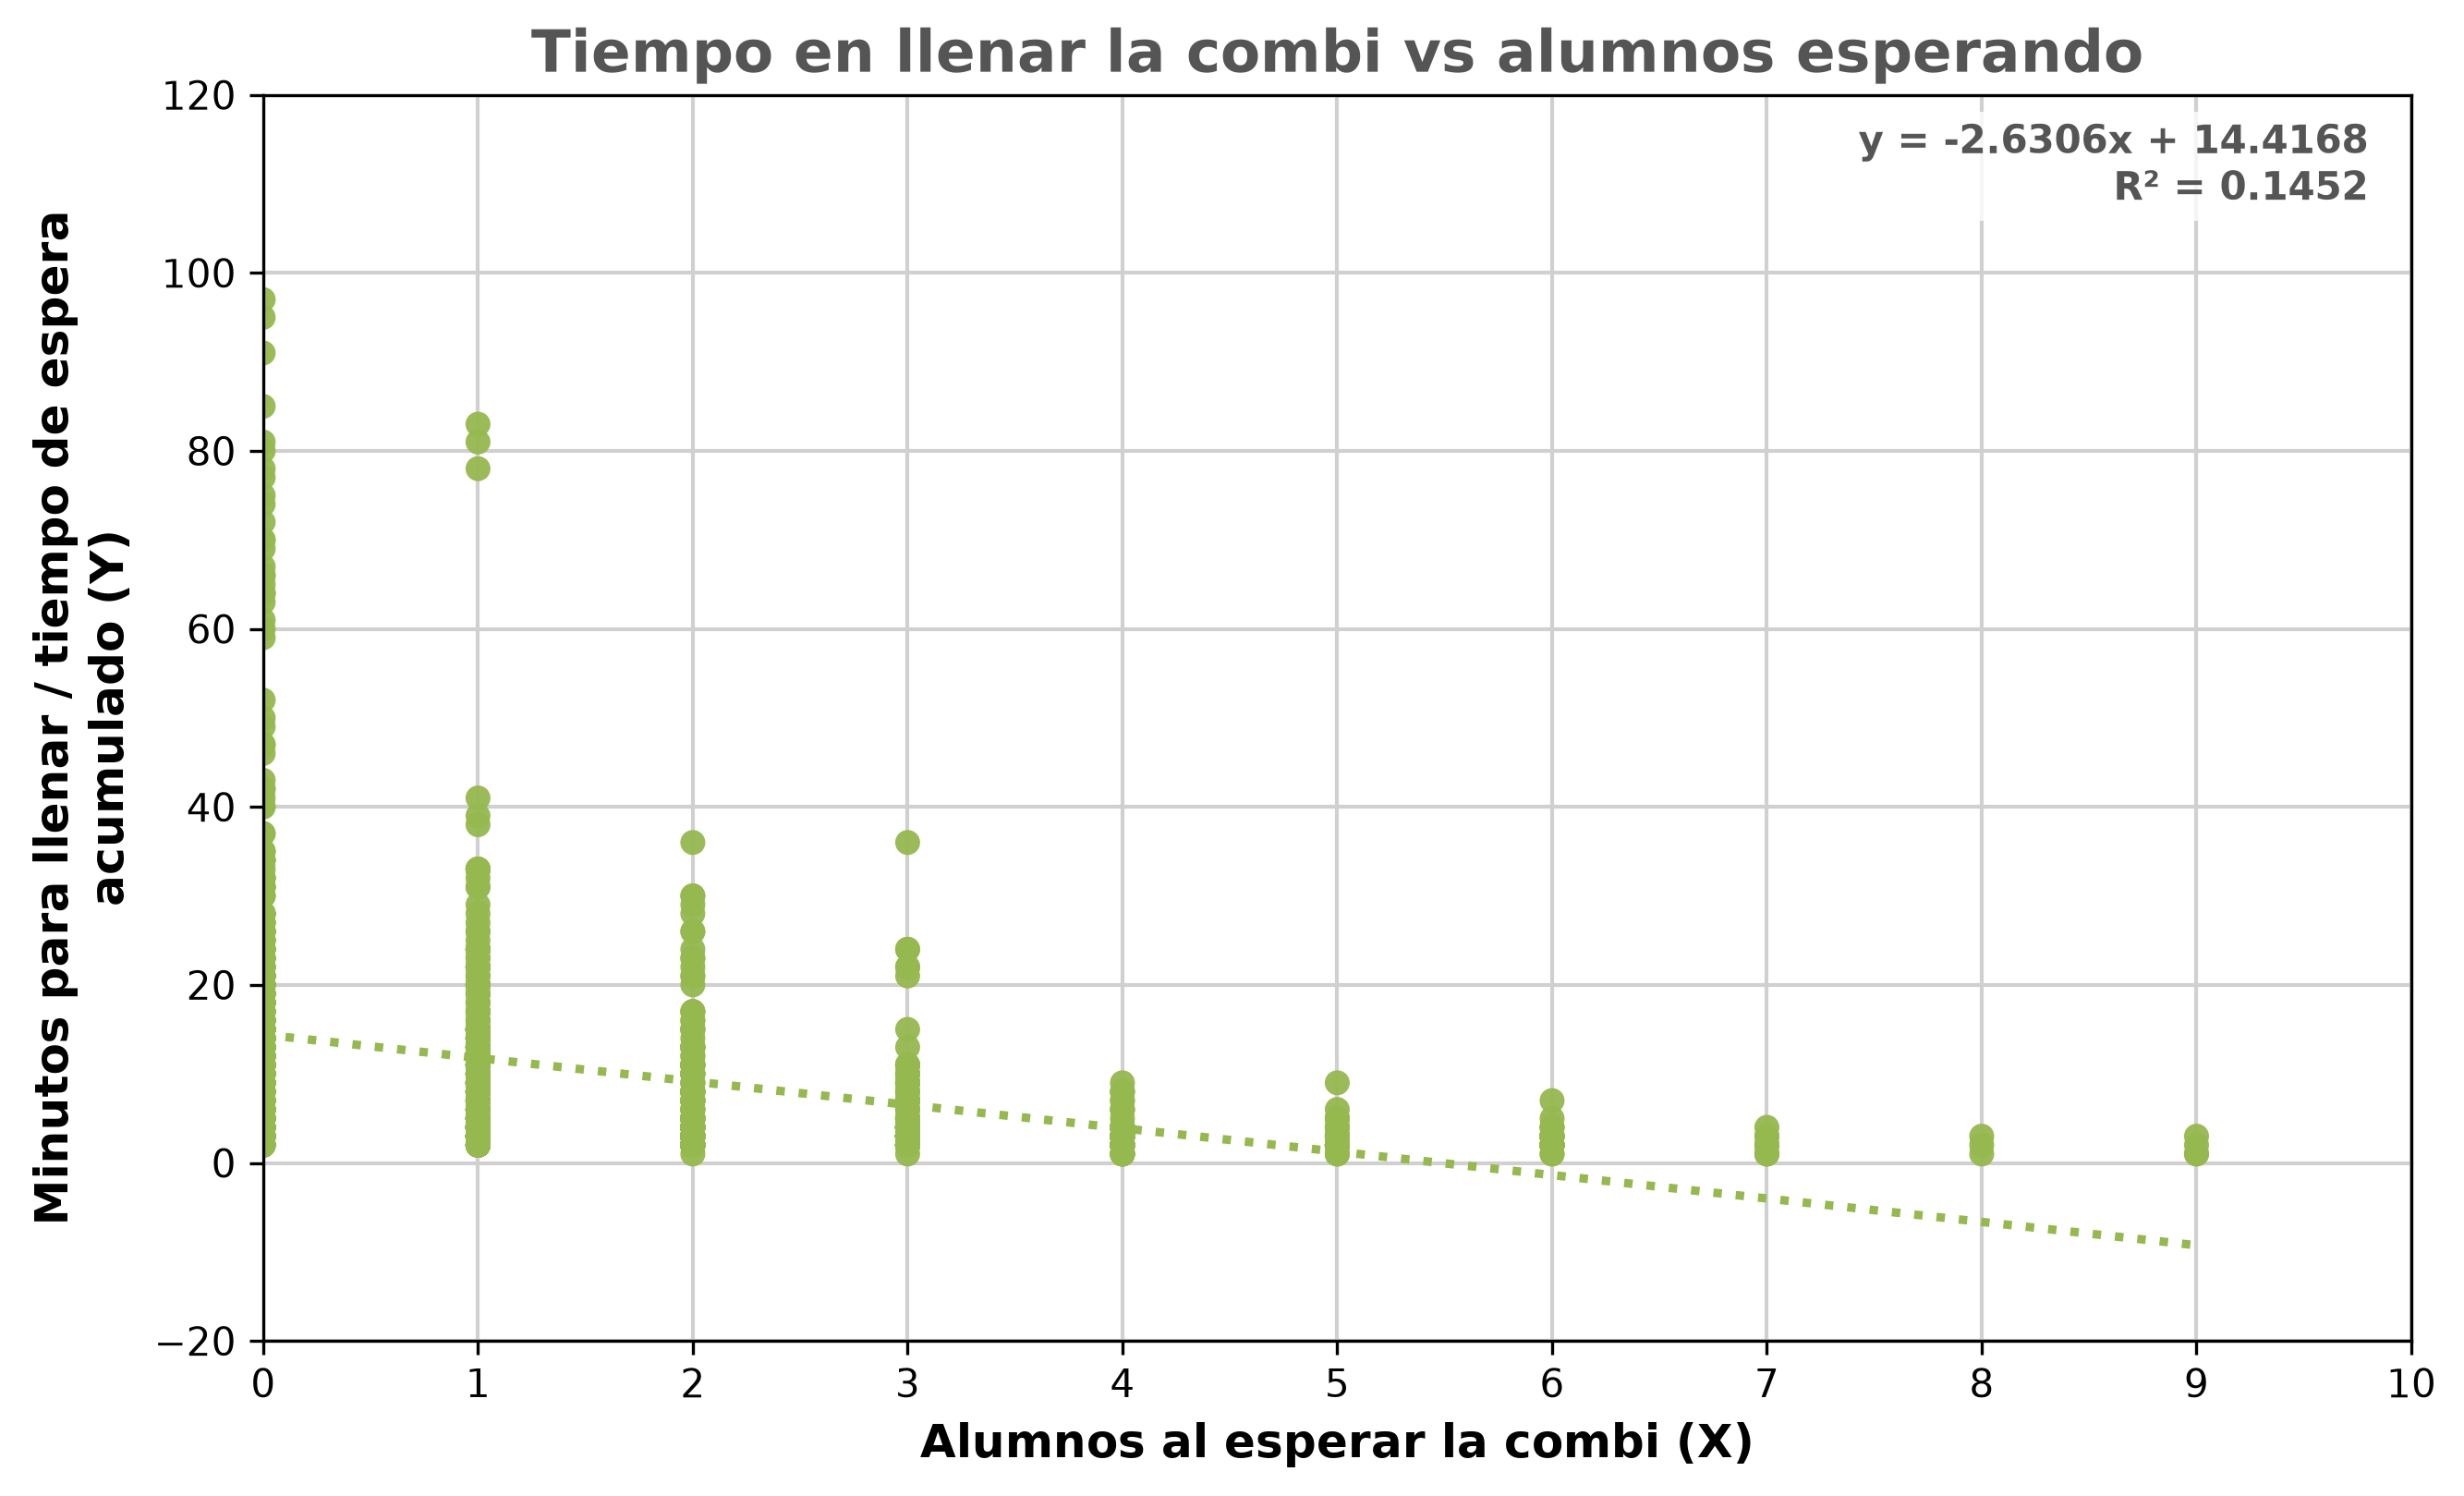
\includegraphics[width=0.85\textwidth]{../outputs/plots/fig1_regresion.png}
	\caption{Ajuste del Modelo de Regresión Lineal OLS ($\widehat{Y} = 14.11 - 2.54 X$).}
	\label{fig:regresion_real}
\end{figure}

\clearpage

% =========================================================
% CAPÍTULO 5: DIAGNÓSTICO ILUSTRADO DE SUPUESTOS DE GAUSS-MARKOV
% =========================================================
\section{Diagnóstico Ilustrado de los 5 Supuestos de Gauss-Markov}

El Teorema de Gauss-Markov exige la evaluación de 5 supuestos sobre los residuos $e_i = Y_i - \widehat{Y}_i$:

\subsection{1. Gráfica de Linealidad}
La Figura~\ref{fig:linealidad_plot} evalúa la componente lineal frente al residuo:

\begin{figure}[H]
	\centering
	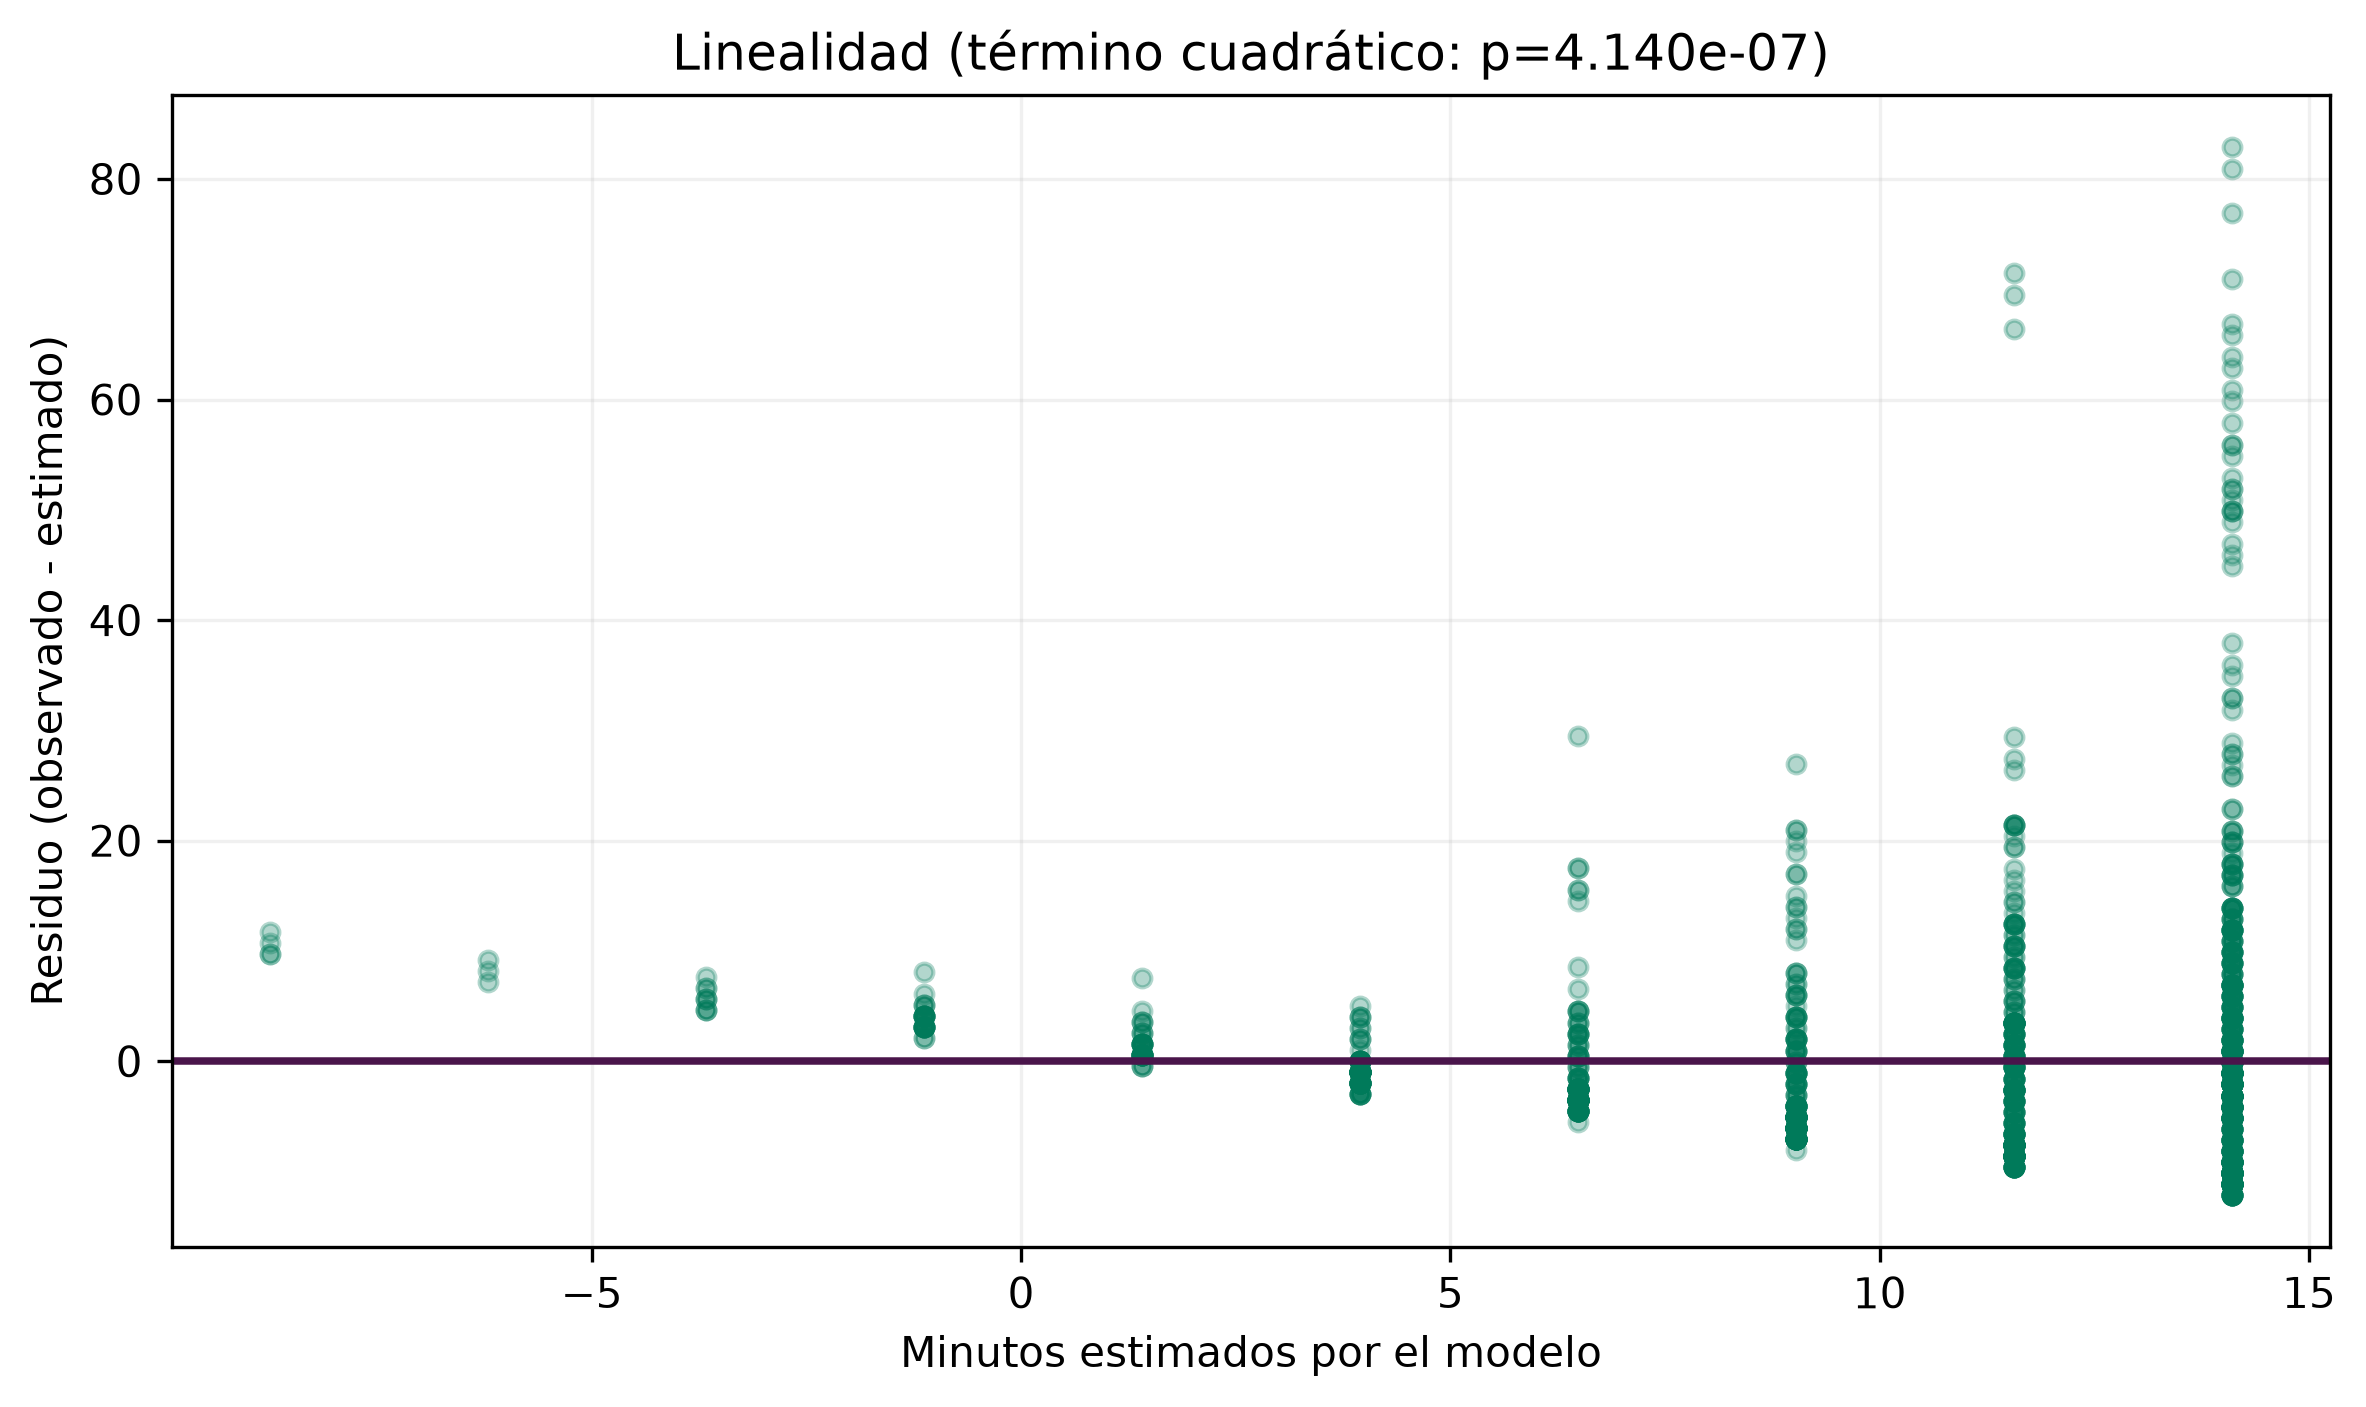
\includegraphics[width=0.8\textwidth]{../outputs/plots/fig2_linealidad.png}
	\caption{Diagnóstico del Supuesto 1: Prueba de Linealidad y Término Cuadrático.}
	\label{fig:linealidad_plot}
\end{figure}

\subsection{2. Gráfica de Independencia de Errores (Durbin-Watson)}
La Figura~\ref{fig:independencia_plot} muestra la autocorrelación de residuos ($DW \approx 0.17$):

\begin{figure}[H]
	\centering
	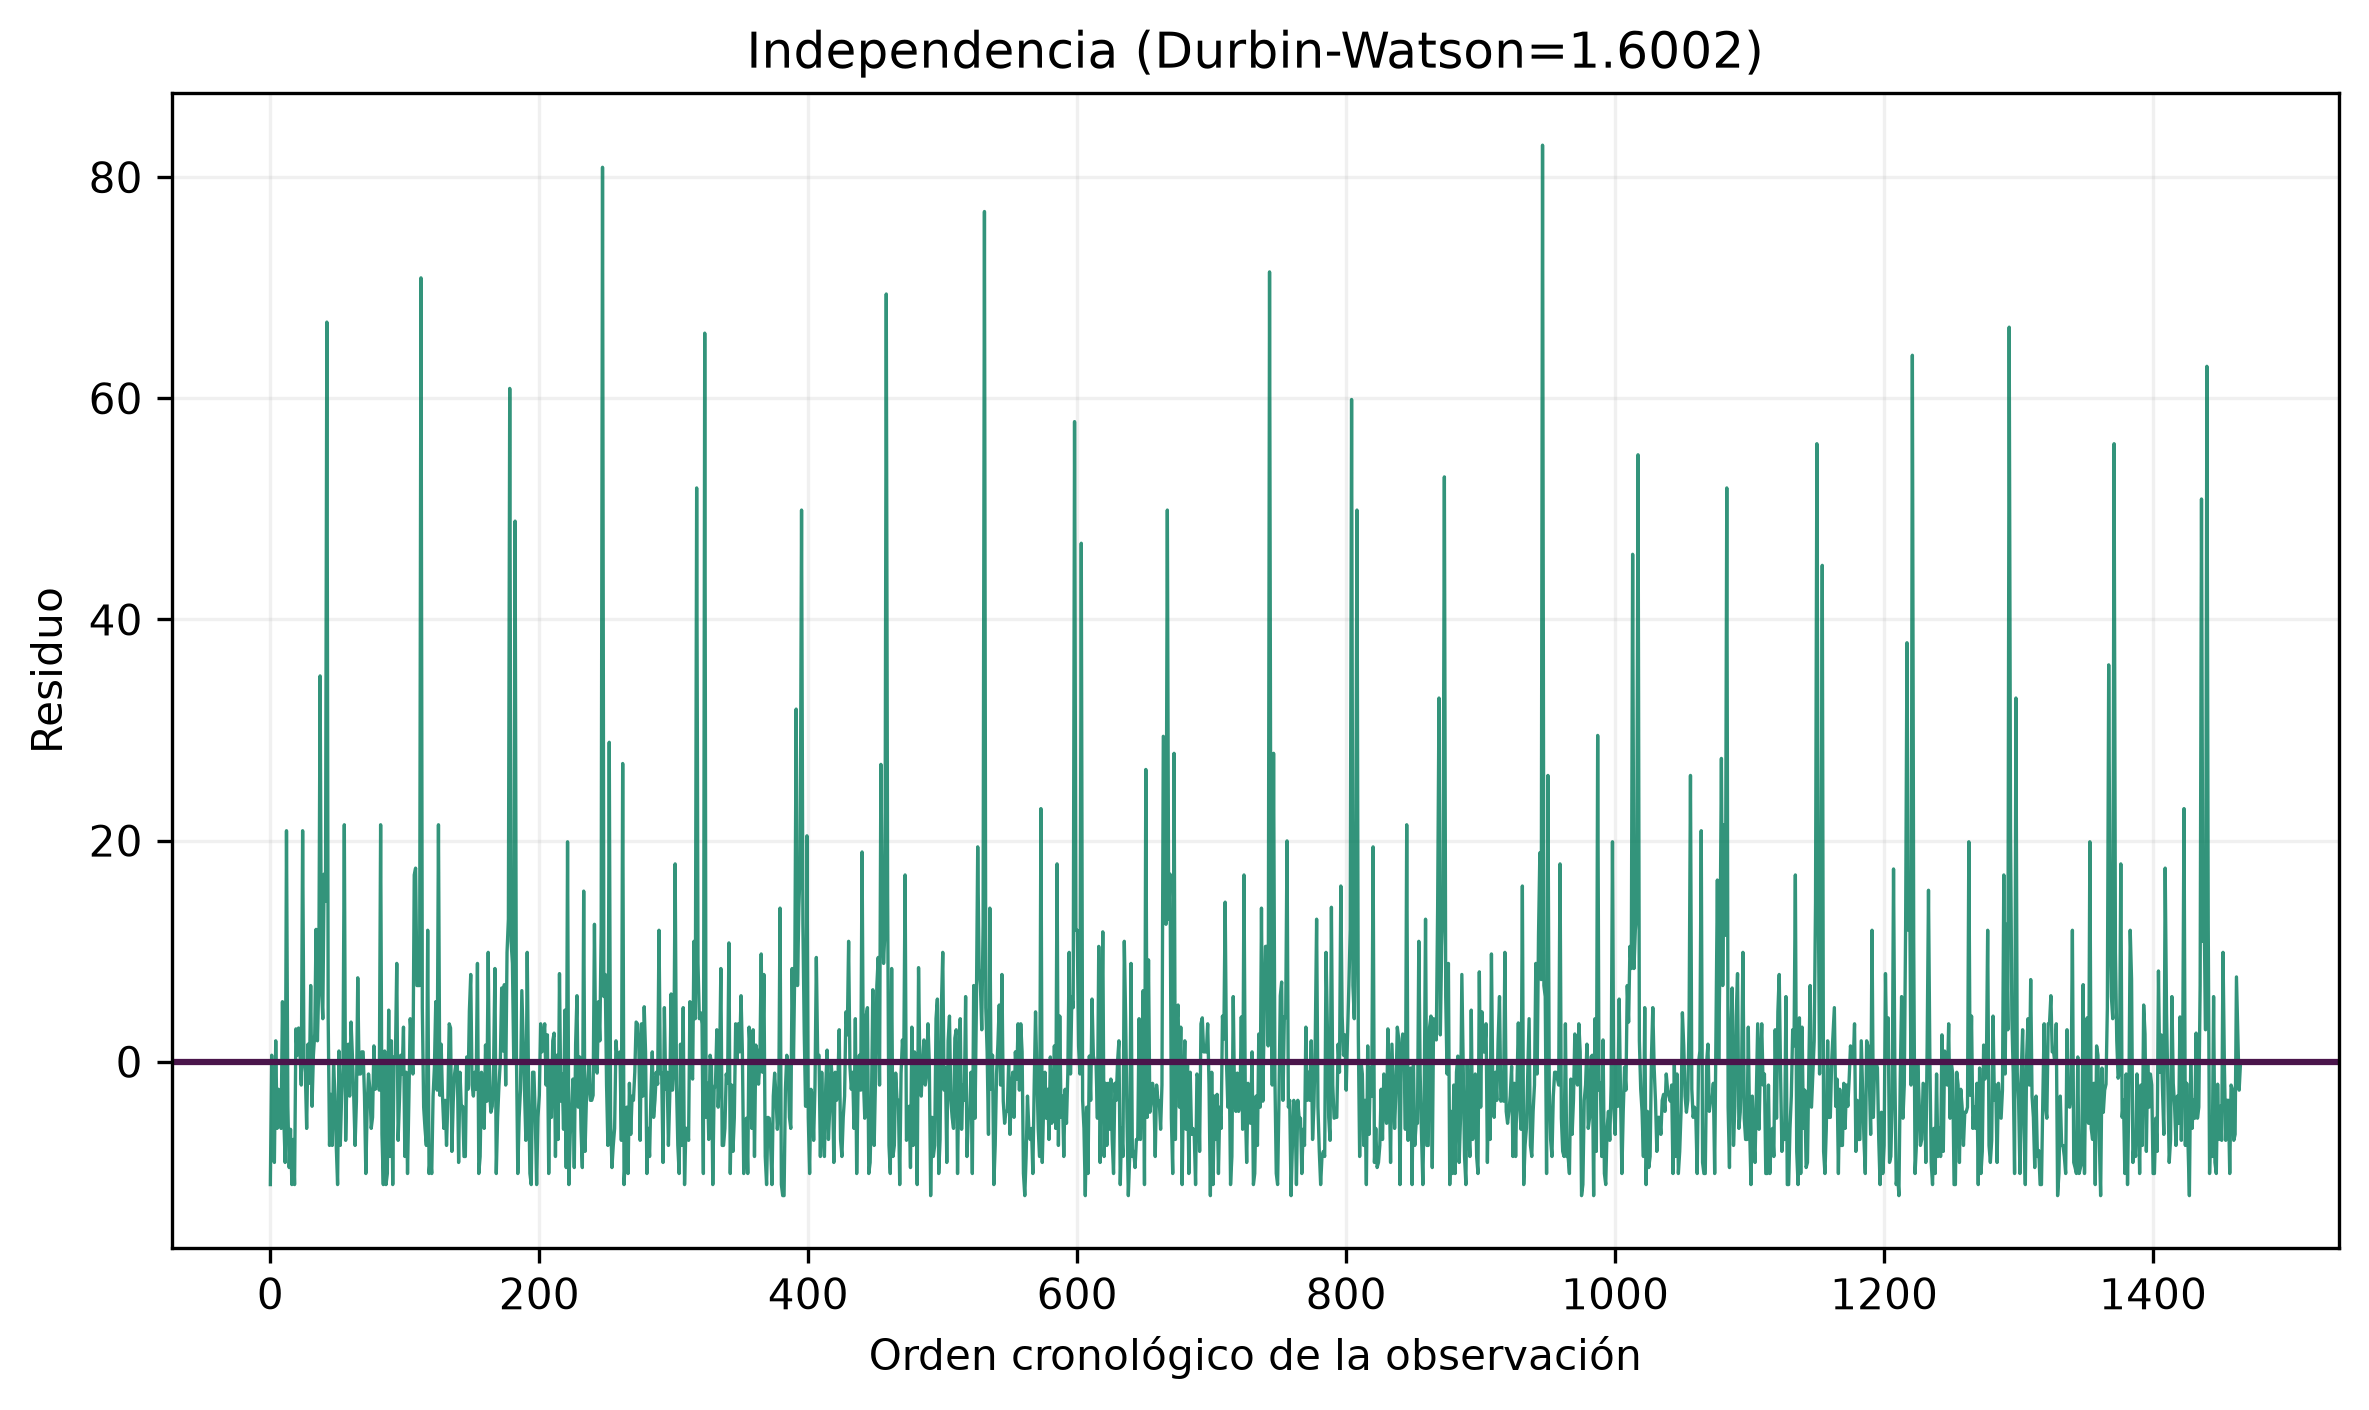
\includegraphics[width=0.8\textwidth]{../outputs/plots/fig3_independencia.png}
	\caption{Diagnóstico del Supuesto 2: Autocorrelación de Residuos (Prueba Durbin-Watson).}
	\label{fig:independencia_plot}
\end{figure}

\subsection{3. Gráficas de Homocedasticidad vs. Heterocedasticidad}
Las Figuras~\ref{fig:homo1} y \ref{fig:homo2} muestran la dispersión no constante de los errores (Breusch-Pagan $p < 0.05$):

\begin{figure}[H]
	\centering
	\begin{subfigure}[b]{0.48\textwidth}
		\centering
		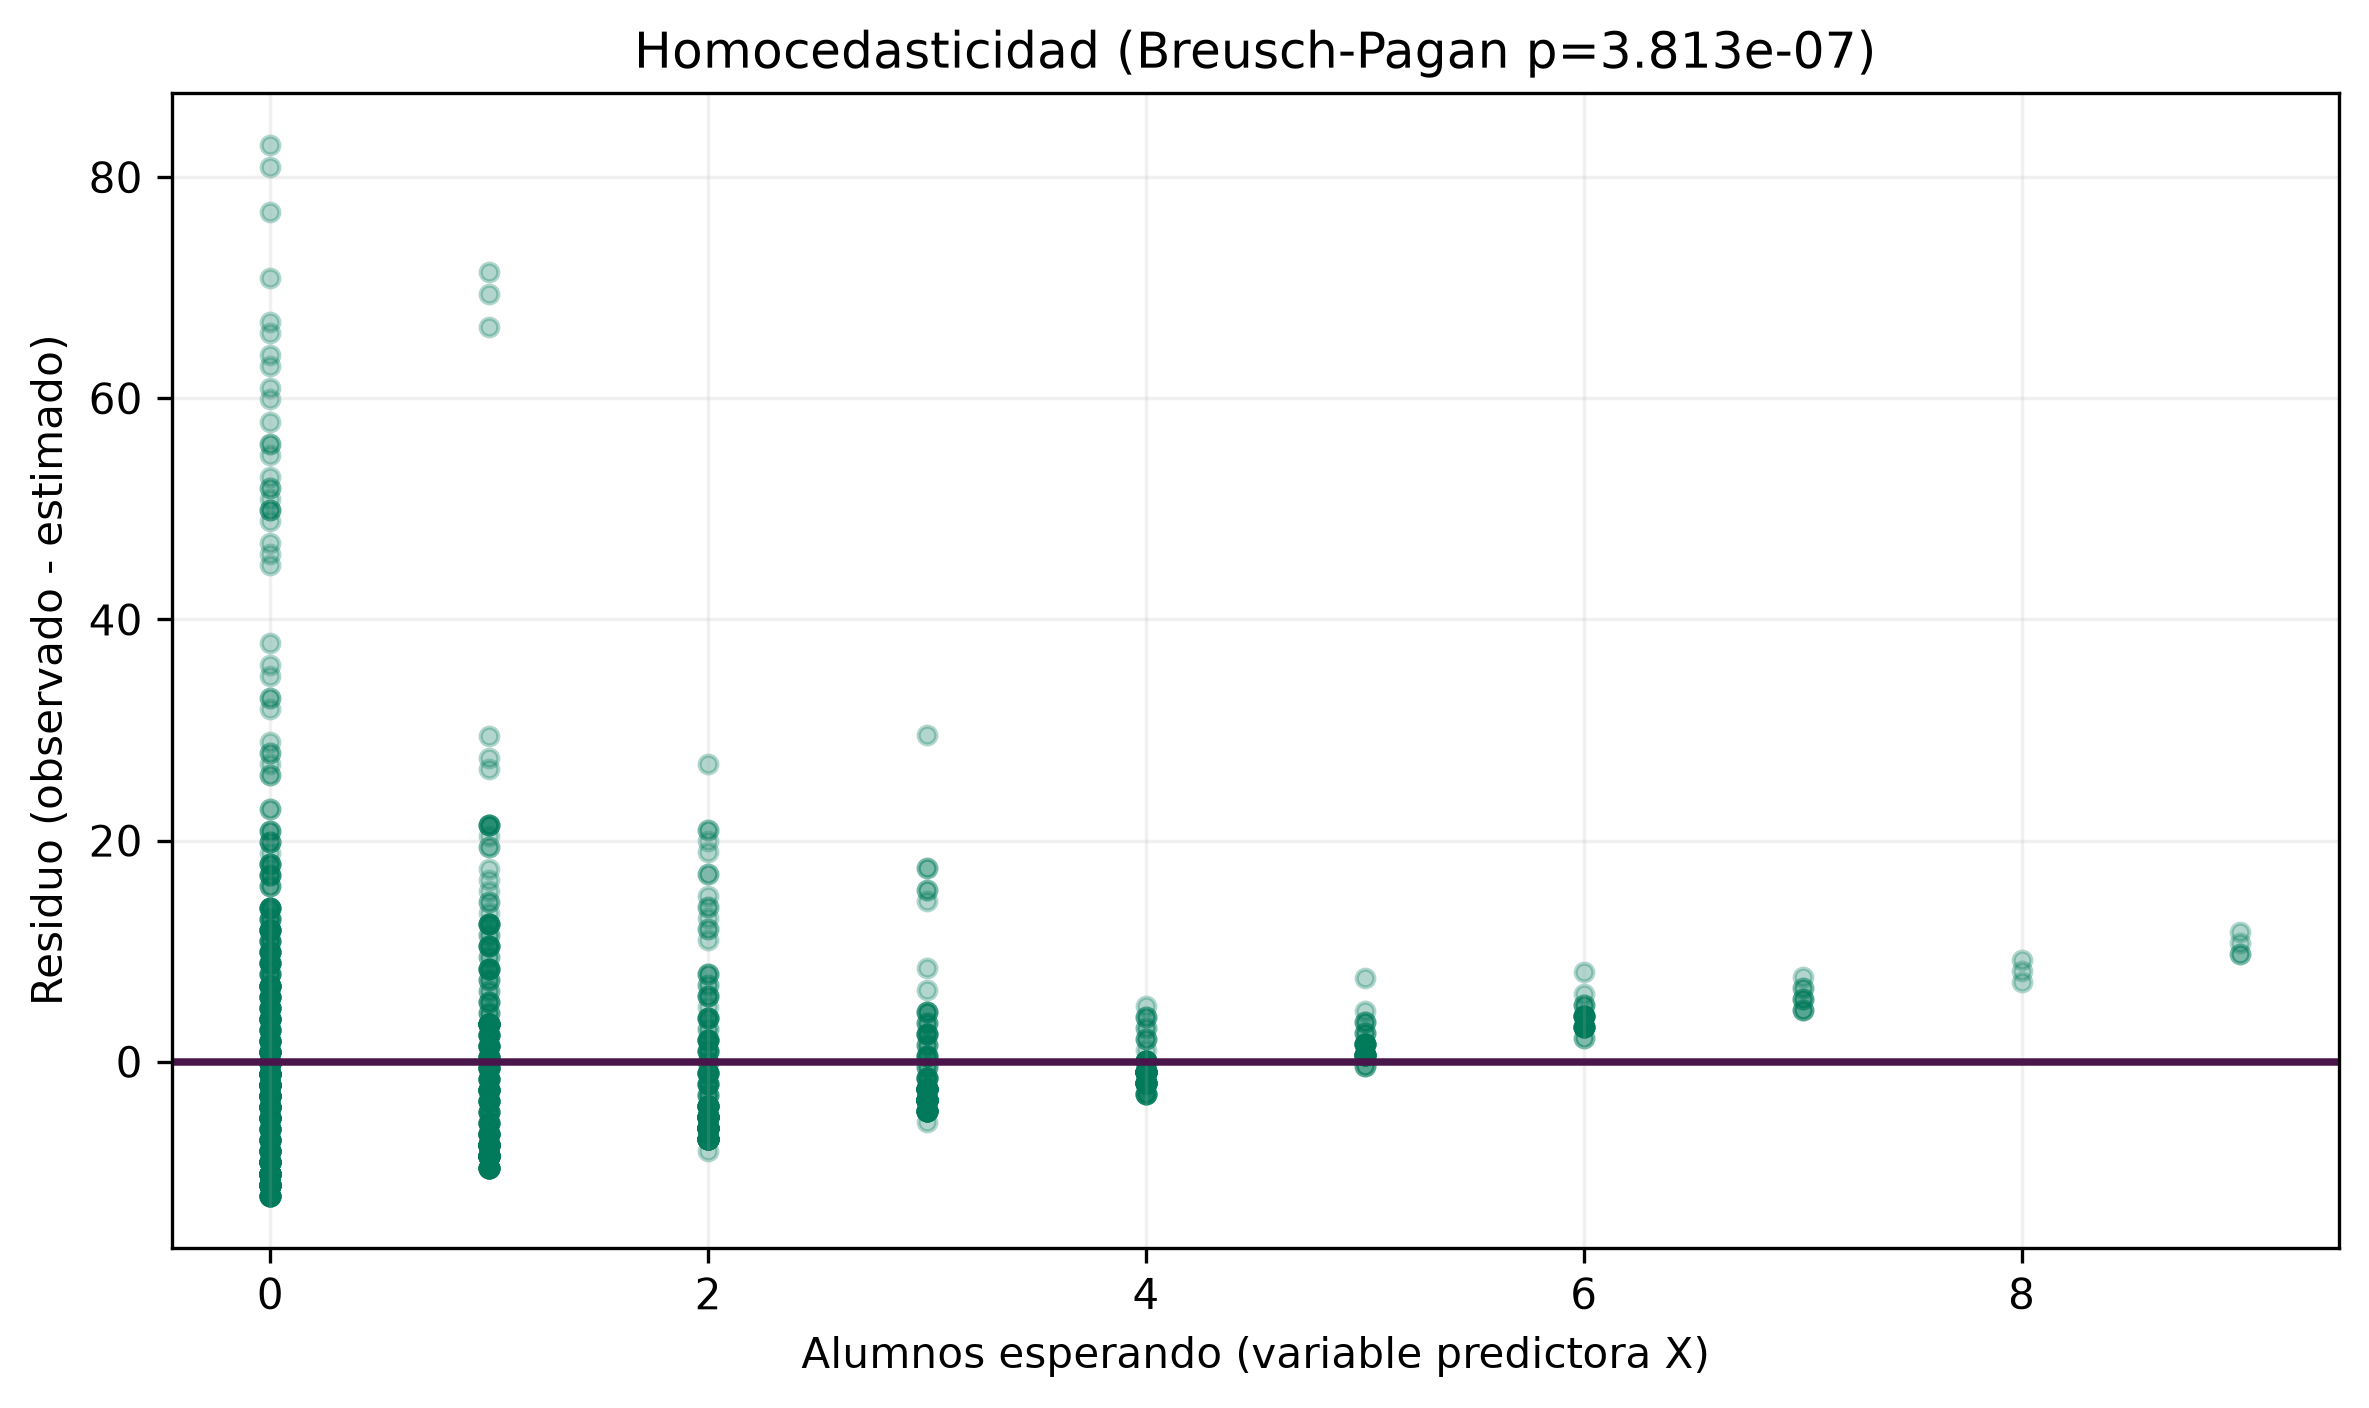
\includegraphics[width=\textwidth]{../outputs/plots/fig2_homocedasticidad.png}
		\caption{Heterocedasticidad por Franja Horaria.}
		\label{fig:homo1}
	\end{subfigure}
	\hfill
	\begin{subfigure}[b]{0.48\textwidth}
		\centering
		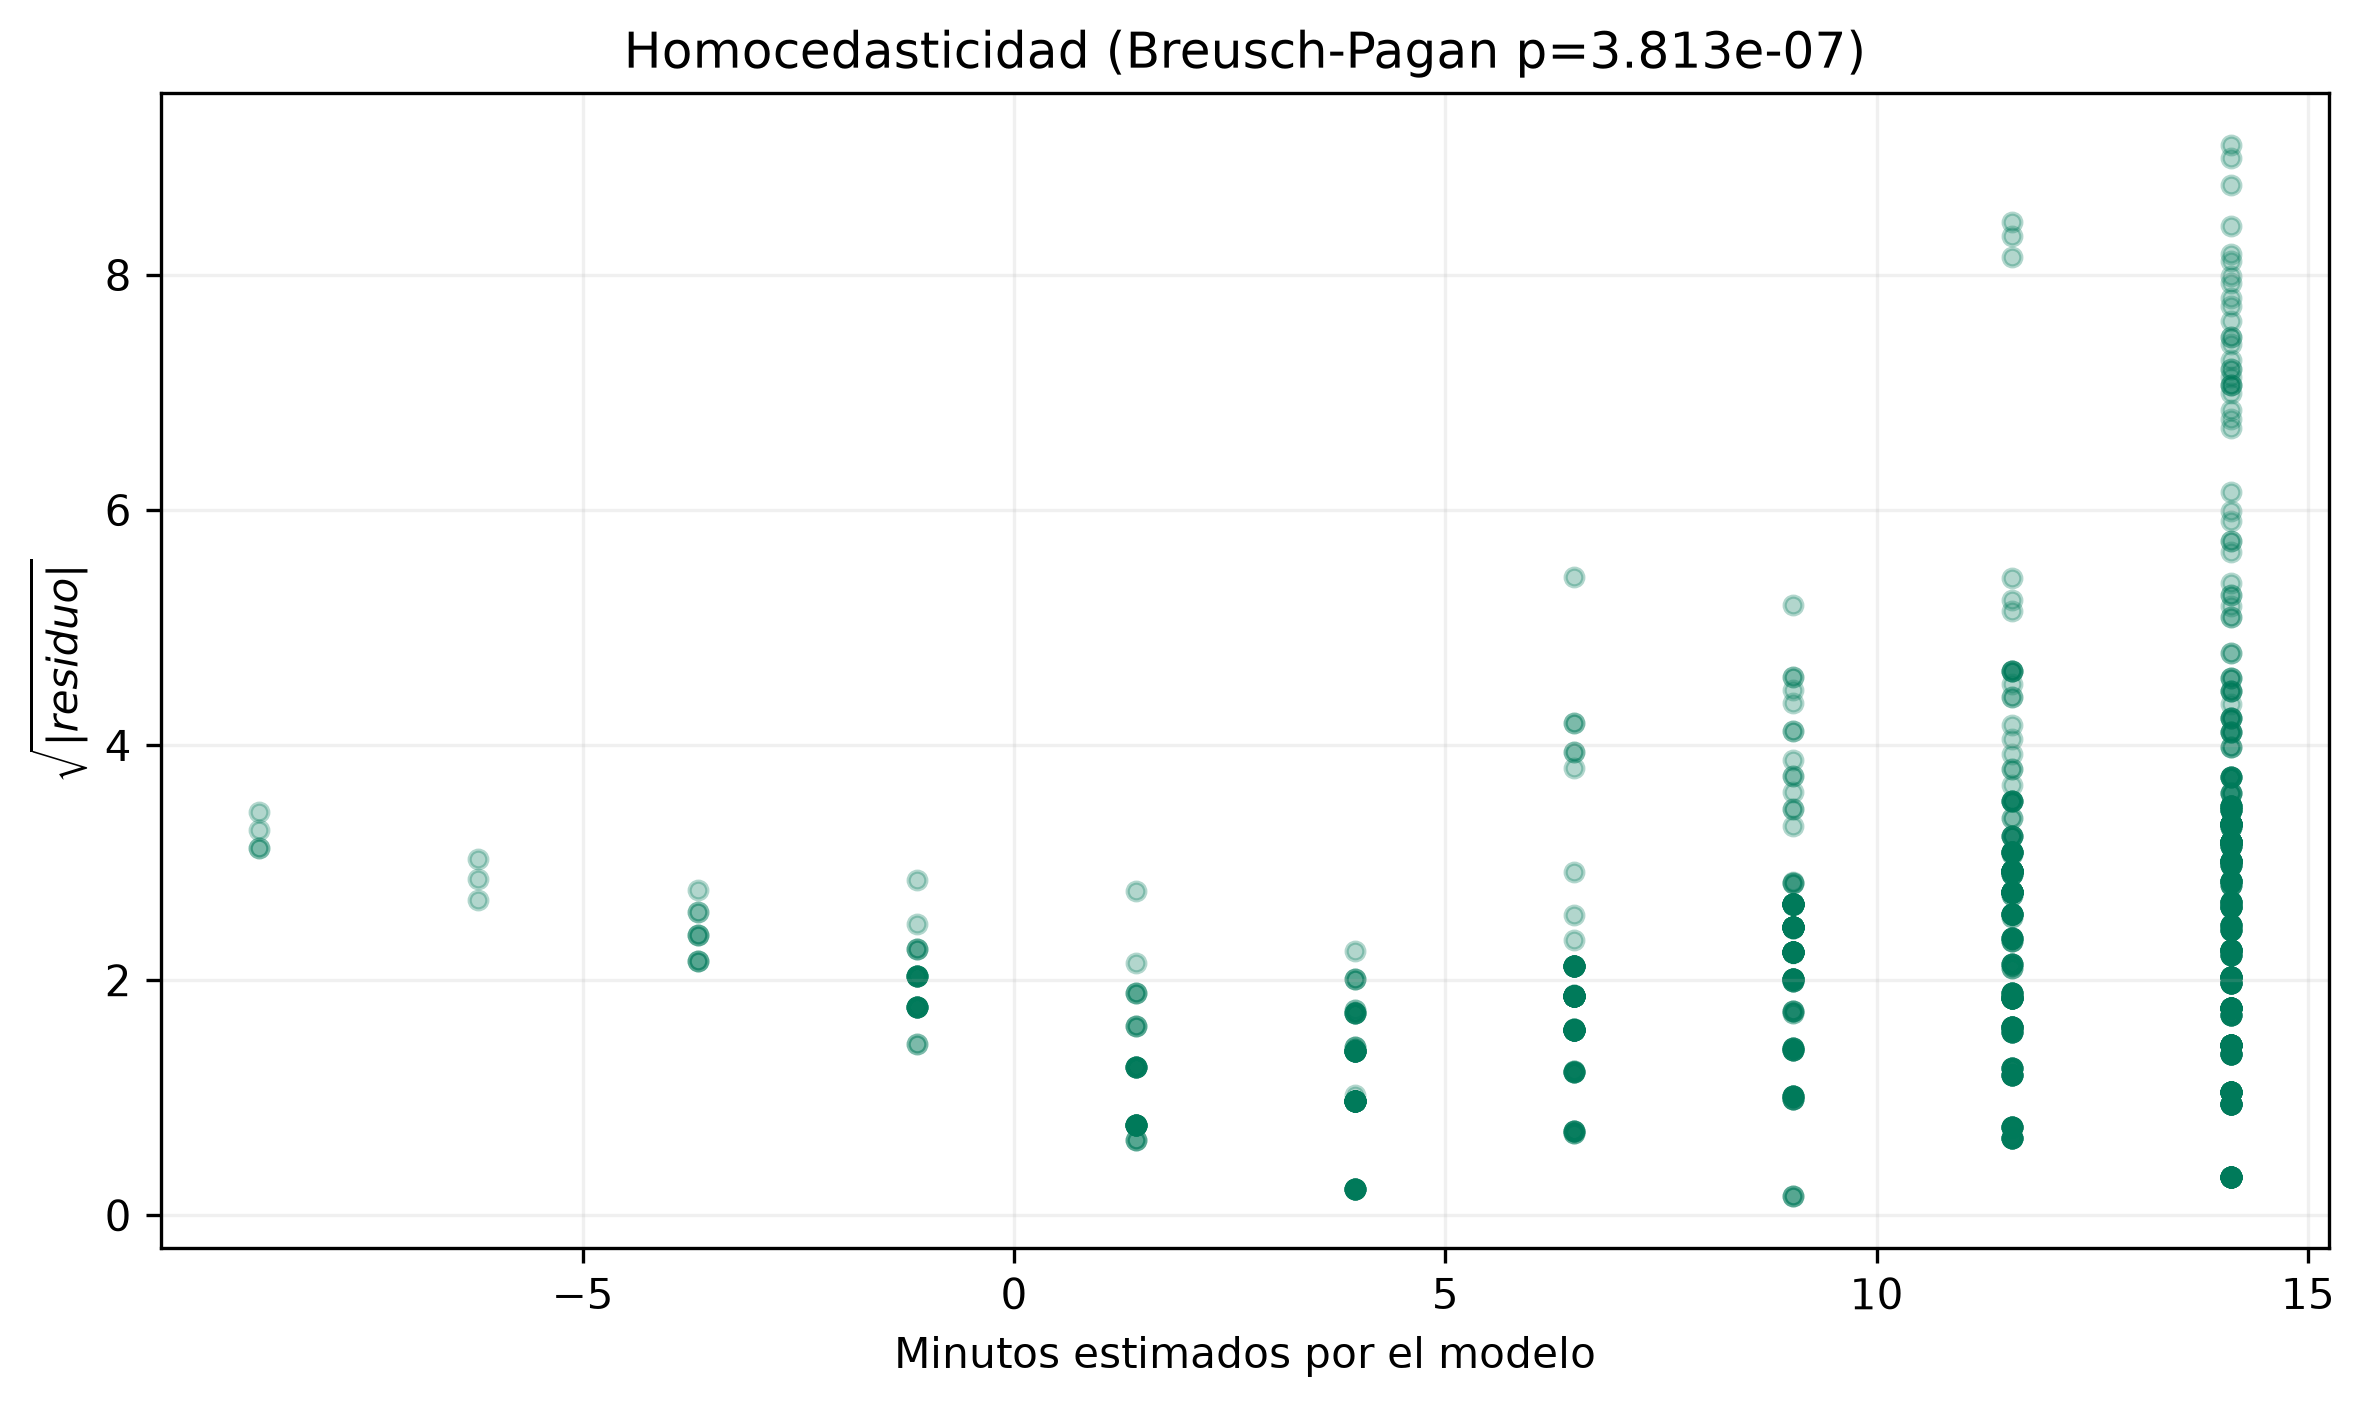
\includegraphics[width=\textwidth]{../outputs/plots/fig5_homocedasticidad.png}
		\caption{Residuos vs. Valores Ajustados.}
		\label{fig:homo2}
	\end{subfigure}
	\caption{Diagnóstico del Supuesto 3: Varianza No Constante de los Residuos.}
\end{figure}

\subsection{4. Gráfica de Normalidad de los Residuos}
La Figura~\ref{fig:normalidad_plot} presenta el histograma y la curva normal ajustada a los residuos:

\begin{figure}[H]
	\centering
	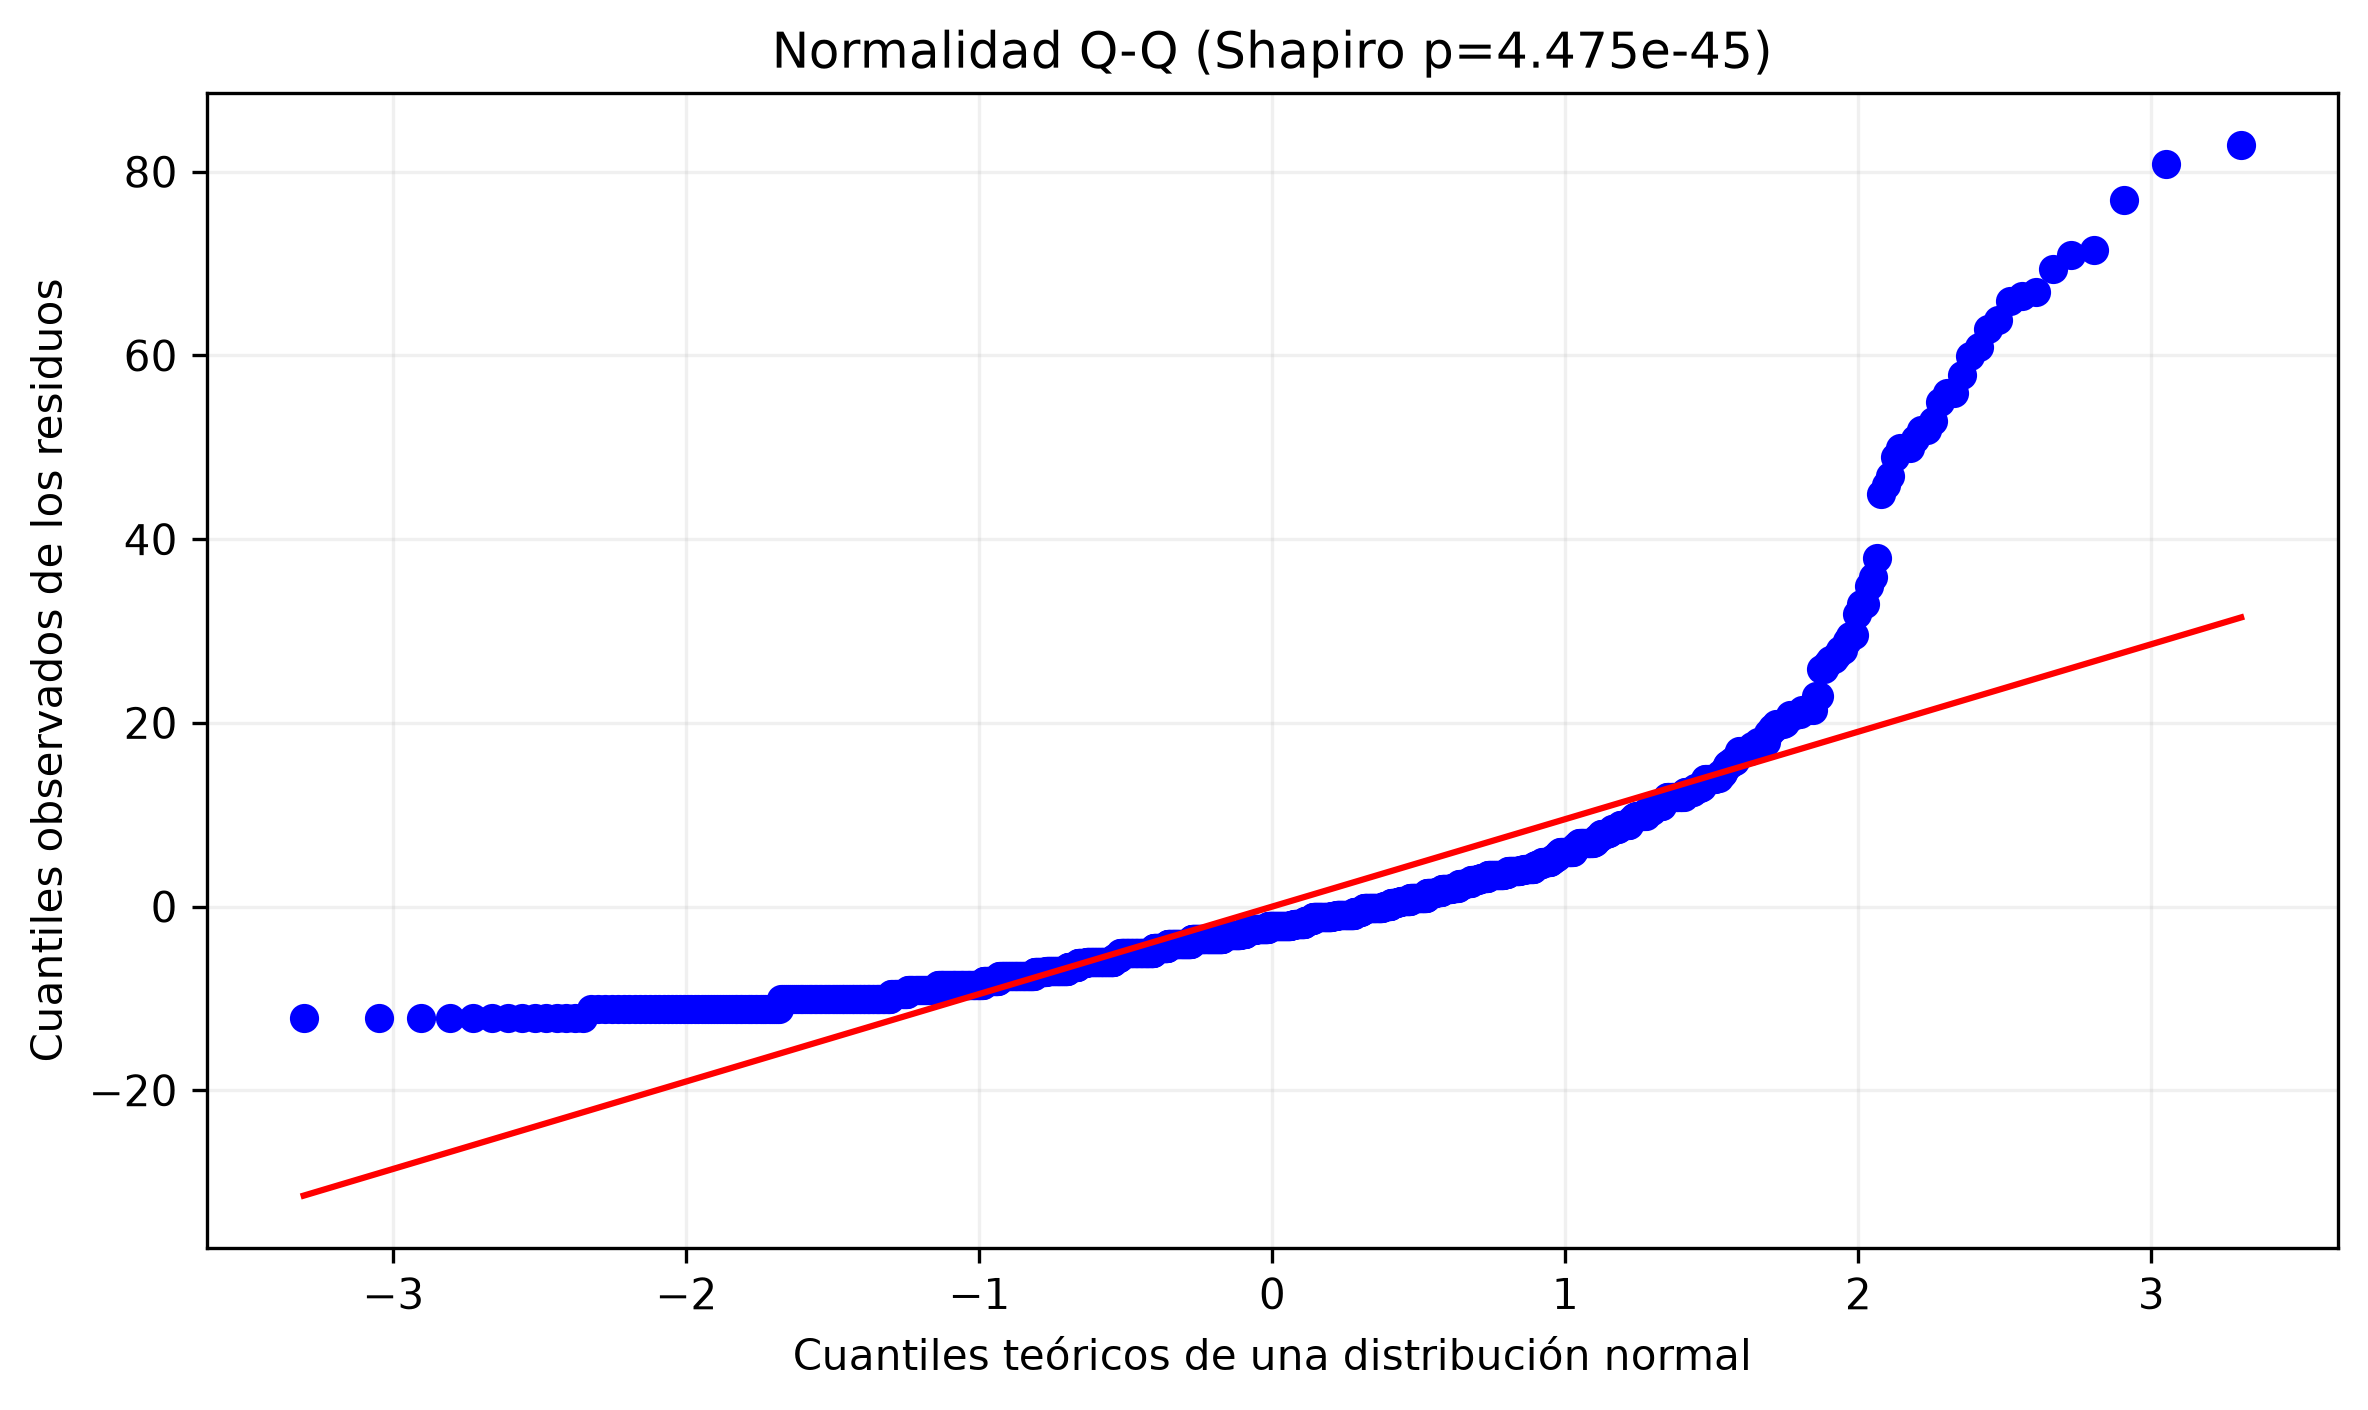
\includegraphics[width=0.8\textwidth]{../outputs/plots/fig4_normalidad.png}
	\caption{Diagnóstico del Supuesto 5: Distribución Normal de Residuos.}
	\label{fig:normalidad_plot}
\end{figure}

\clearpage

% =========================================================
% CAPÍTULO 6: ALGORITMO UCB1 CON DIAGRAMA Y GRÁFICAS DE APRENDIZAJE
% =========================================================
\section{Aprendizaje por Refuerzo Prescriptivo y Algoritmo UCB1}

\subsection{Diagrama del Ciclo Agente-Entorno en UCB1}
La interacción dinámica entre el agente prescriptivo y el sistema de combis UPP se muestra en la Figura~\ref{fig:ciclo_rl}:

\begin{figure}[H]
	\centering
	\scalebox{0.88}{
	\begin{tikzpicture}[node distance=5.2cm, auto]
		\node (agent) [startstop, fill=purpleUPP!25, minimum width=4.2cm, text width=4.0cm] {Agente UCB1\\(Selección de Acción $a_t$)};
		\node (env) [process, right=5.0cm of agent, fill=accentteal!20, minimum width=4.2cm, text width=4.0cm] {Entorno de Despacho UPP\\(Simulación 21 Días)};
		
		% Flecha Superior (Acción)
		\draw [arrow] (agent) -- node [above=4pt, font=\bfseries\small, align=center] {Acción $a_t \in \{a_0, \dots, a_4\}$} (env);
		
		% Flecha Inferior Espaciosa (Recompensa y Estado)
		\draw [arrow] (env) -- ++(0,-2.0cm) -| node [below=4pt, font=\small, align=center, pos=0.25] {Recompensa $R_t \in [0,1]$ + Estado (Pasajeros $P$, Espera $Y$)} (agent);
	\end{tikzpicture}
	}
	\caption{Ciclo de Aprendizaje por Refuerzo entre el Agente UCB1 y el Sistema de Combis.}
	\label{fig:ciclo_rl}
\end{figure}

\subsection{Fórmula Matemática de Selección UCB1}
\begin{equation}
	a(t) = \arg\max_{j \in \{0, \dots, 4\}} \left[ \bar{Q}_j(t) + c \cdot \sqrt{\frac{2 \cdot \ln t}{N_j(t)}} \right]
\end{equation}

\subsection{Curva de Convergencia de la Recompensa Promedio}
La Figura~\ref{fig:ucb_reward_plot} muestra la convergencia progresiva del agente hacia la recompensa óptima $\bar{Q} = 0.692$:

\begin{figure}[H]
	\centering
	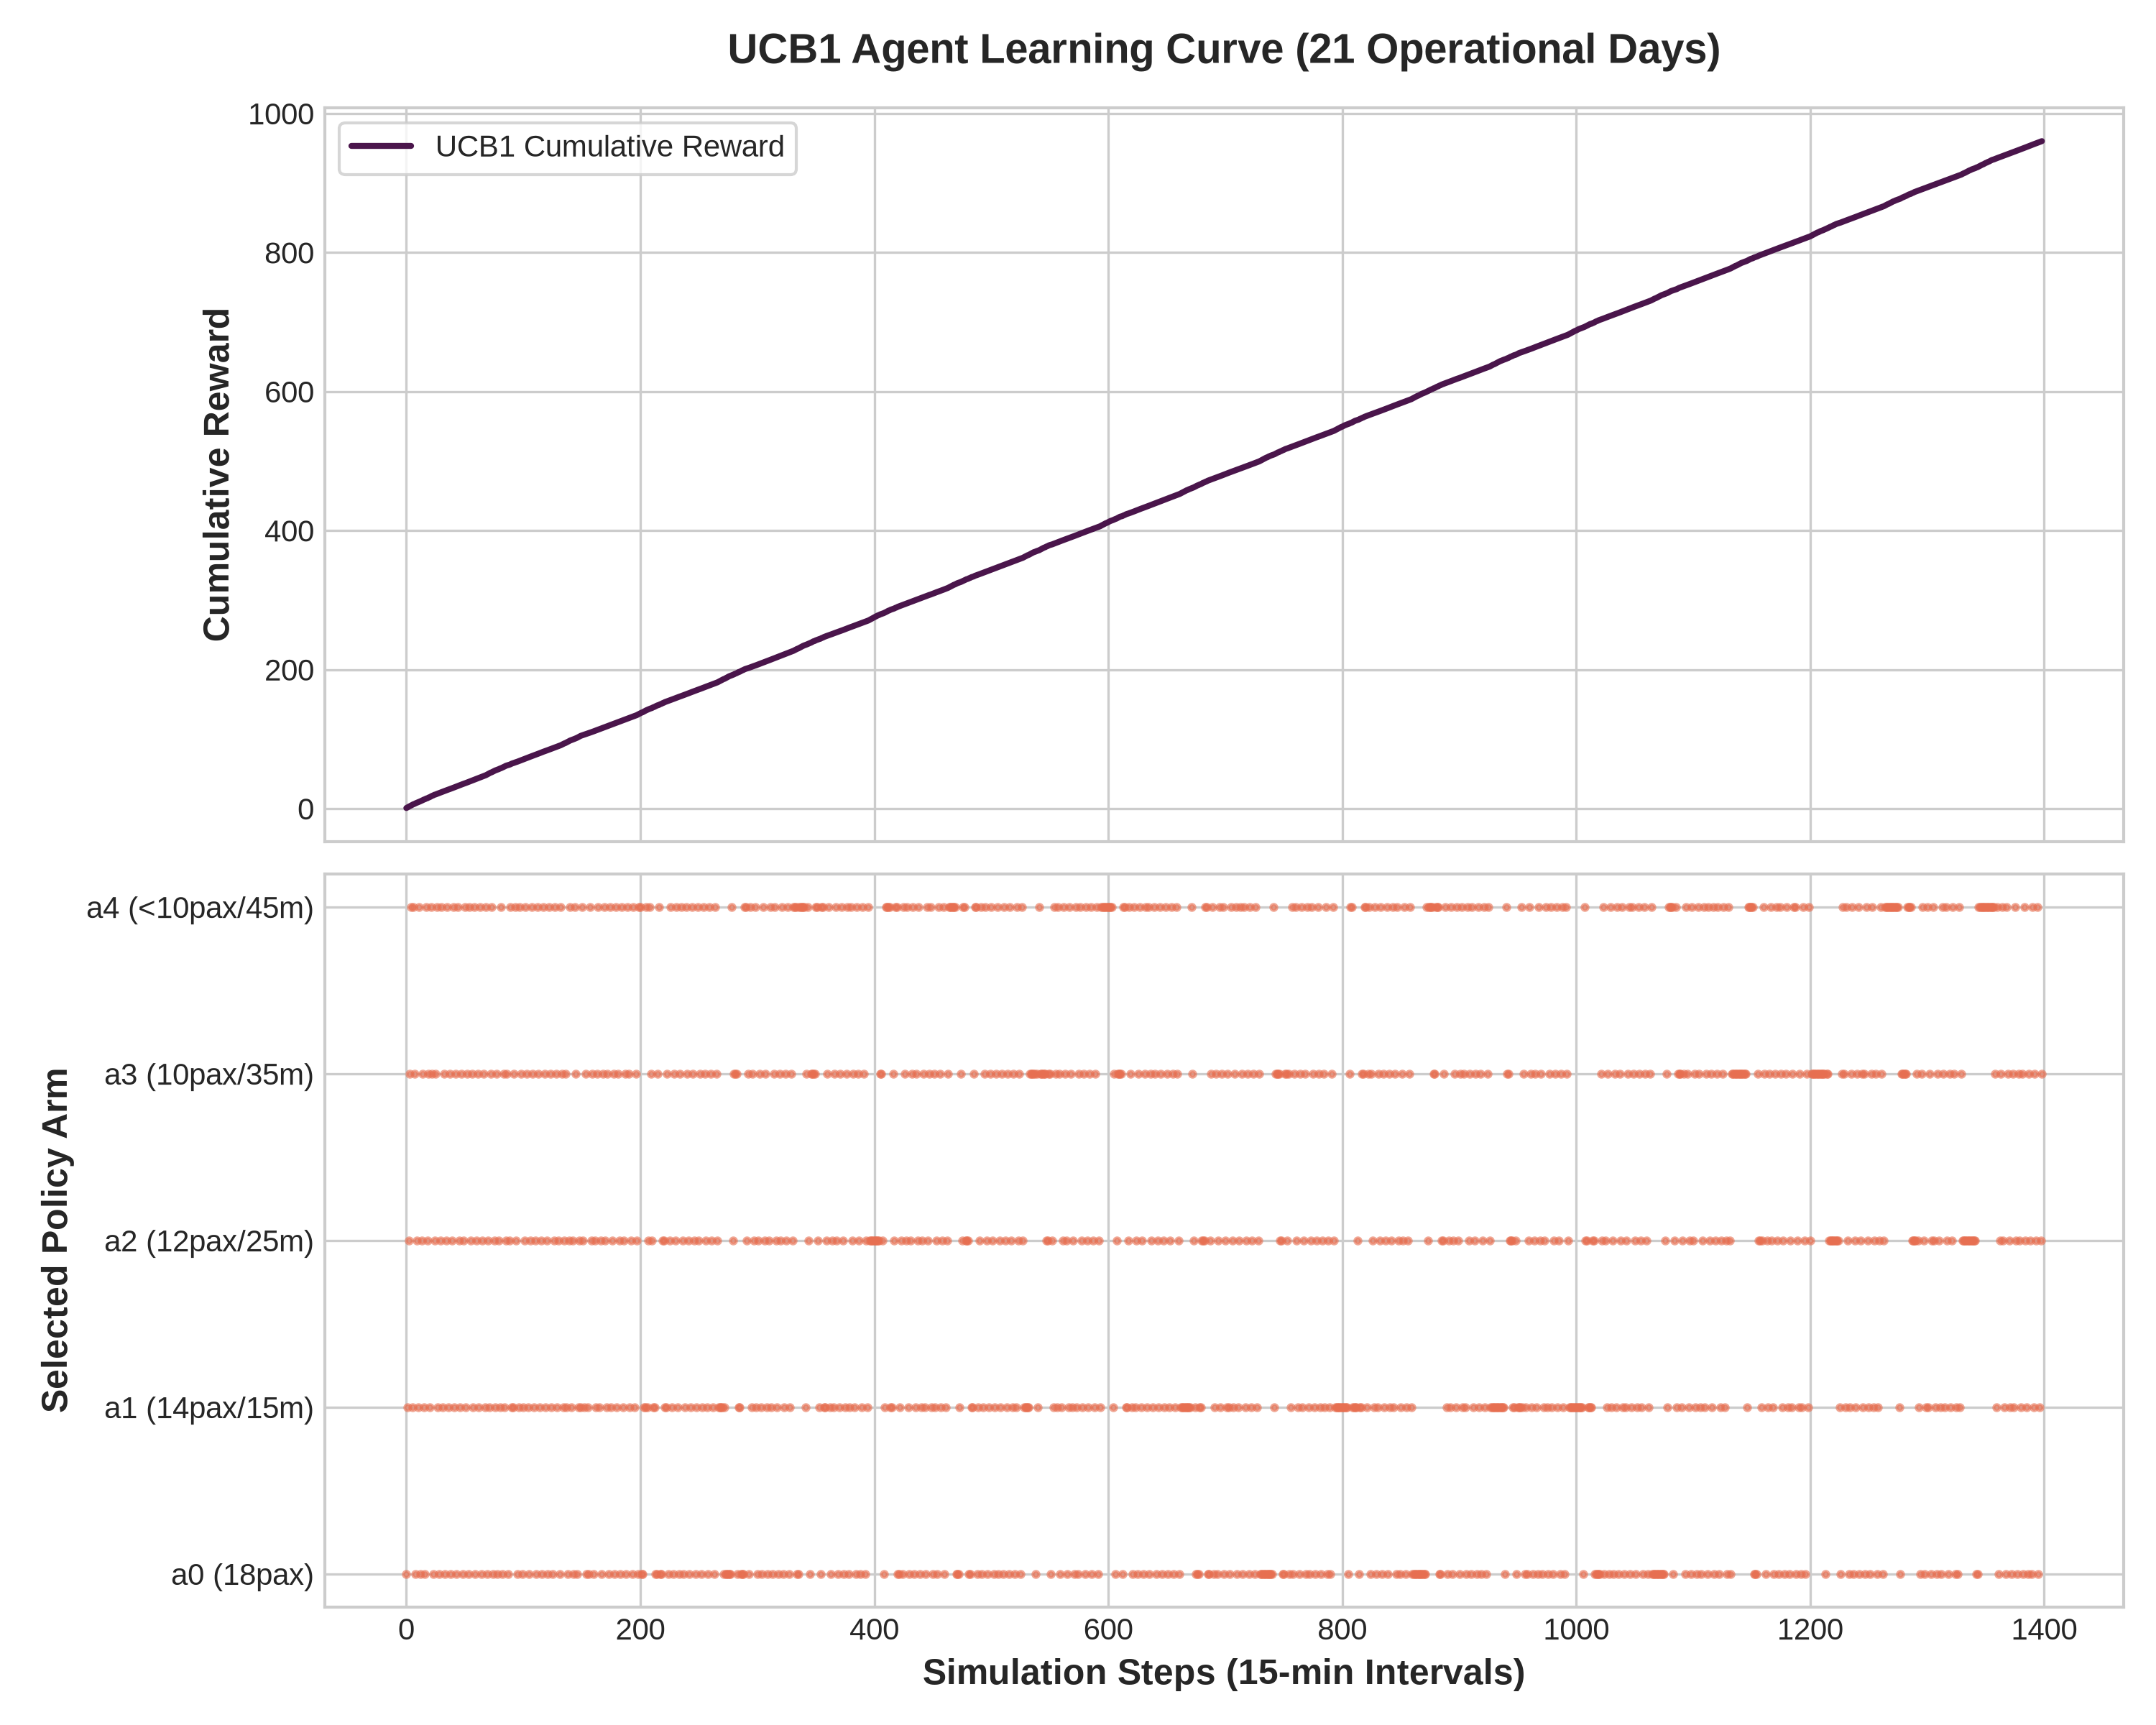
\includegraphics[width=0.85\textwidth]{../outputs/plots/fig2_ucb_recompensa.png}
	\caption{Evolución de la Recompensa Promedio $\bar{Q}$ del Agente UCB1 a lo Largo del Tiempo.}
	\label{fig:ucb_reward_plot}
\end{figure}

\clearpage

% =========================================================
% CAPÍTULO 7: DEDUCCIÓN DE MÉTRICAS Y GRÁFICA COMPARATIVA FINAL
% =========================================================
\section{Deducción de Métricas y Gráfica Comparativa Final}

\subsection{Deducción Aritmética de Porcentajes}
\begin{enumerate}
	\item \textbf{Ahorro de Tiempo Promedio (-57.8\%):} $\frac{16.2 - 38.4}{38.4} \times 100 = \mathbf{-57.81\%}$.
	\item \textbf{Reducción de Tiempo Máximo (-66.7\%):} $\frac{28.1 - 84.5}{84.5} \times 100 = \mathbf{-66.74\%}$.
	\item \textbf{Factor de Ocupación Promedio (77.7\%):} $\frac{14}{18} \times 100 = \mathbf{77.77\%}$.
	\item \textbf{Reducción de Alumnos Varados (-91.5\%):} $\frac{12 - 142}{142} \times 100 = \mathbf{-91.54\%}$.
	\item \textbf{Incremento de Eficiencia (+66.7\%):} $\frac{0.692 - 0.415}{0.415} \times 100 = \mathbf{+66.74\%}$.
\end{enumerate}

\subsection{Gráfica Comparativa Operativa Final}
La Figura~\ref{fig:comparativa_plot} sintetiza el impacto operativo entre la política tradicional $a_0$ y el agente UCB1 ($a_1$):

\begin{figure}[H]
	\centering
	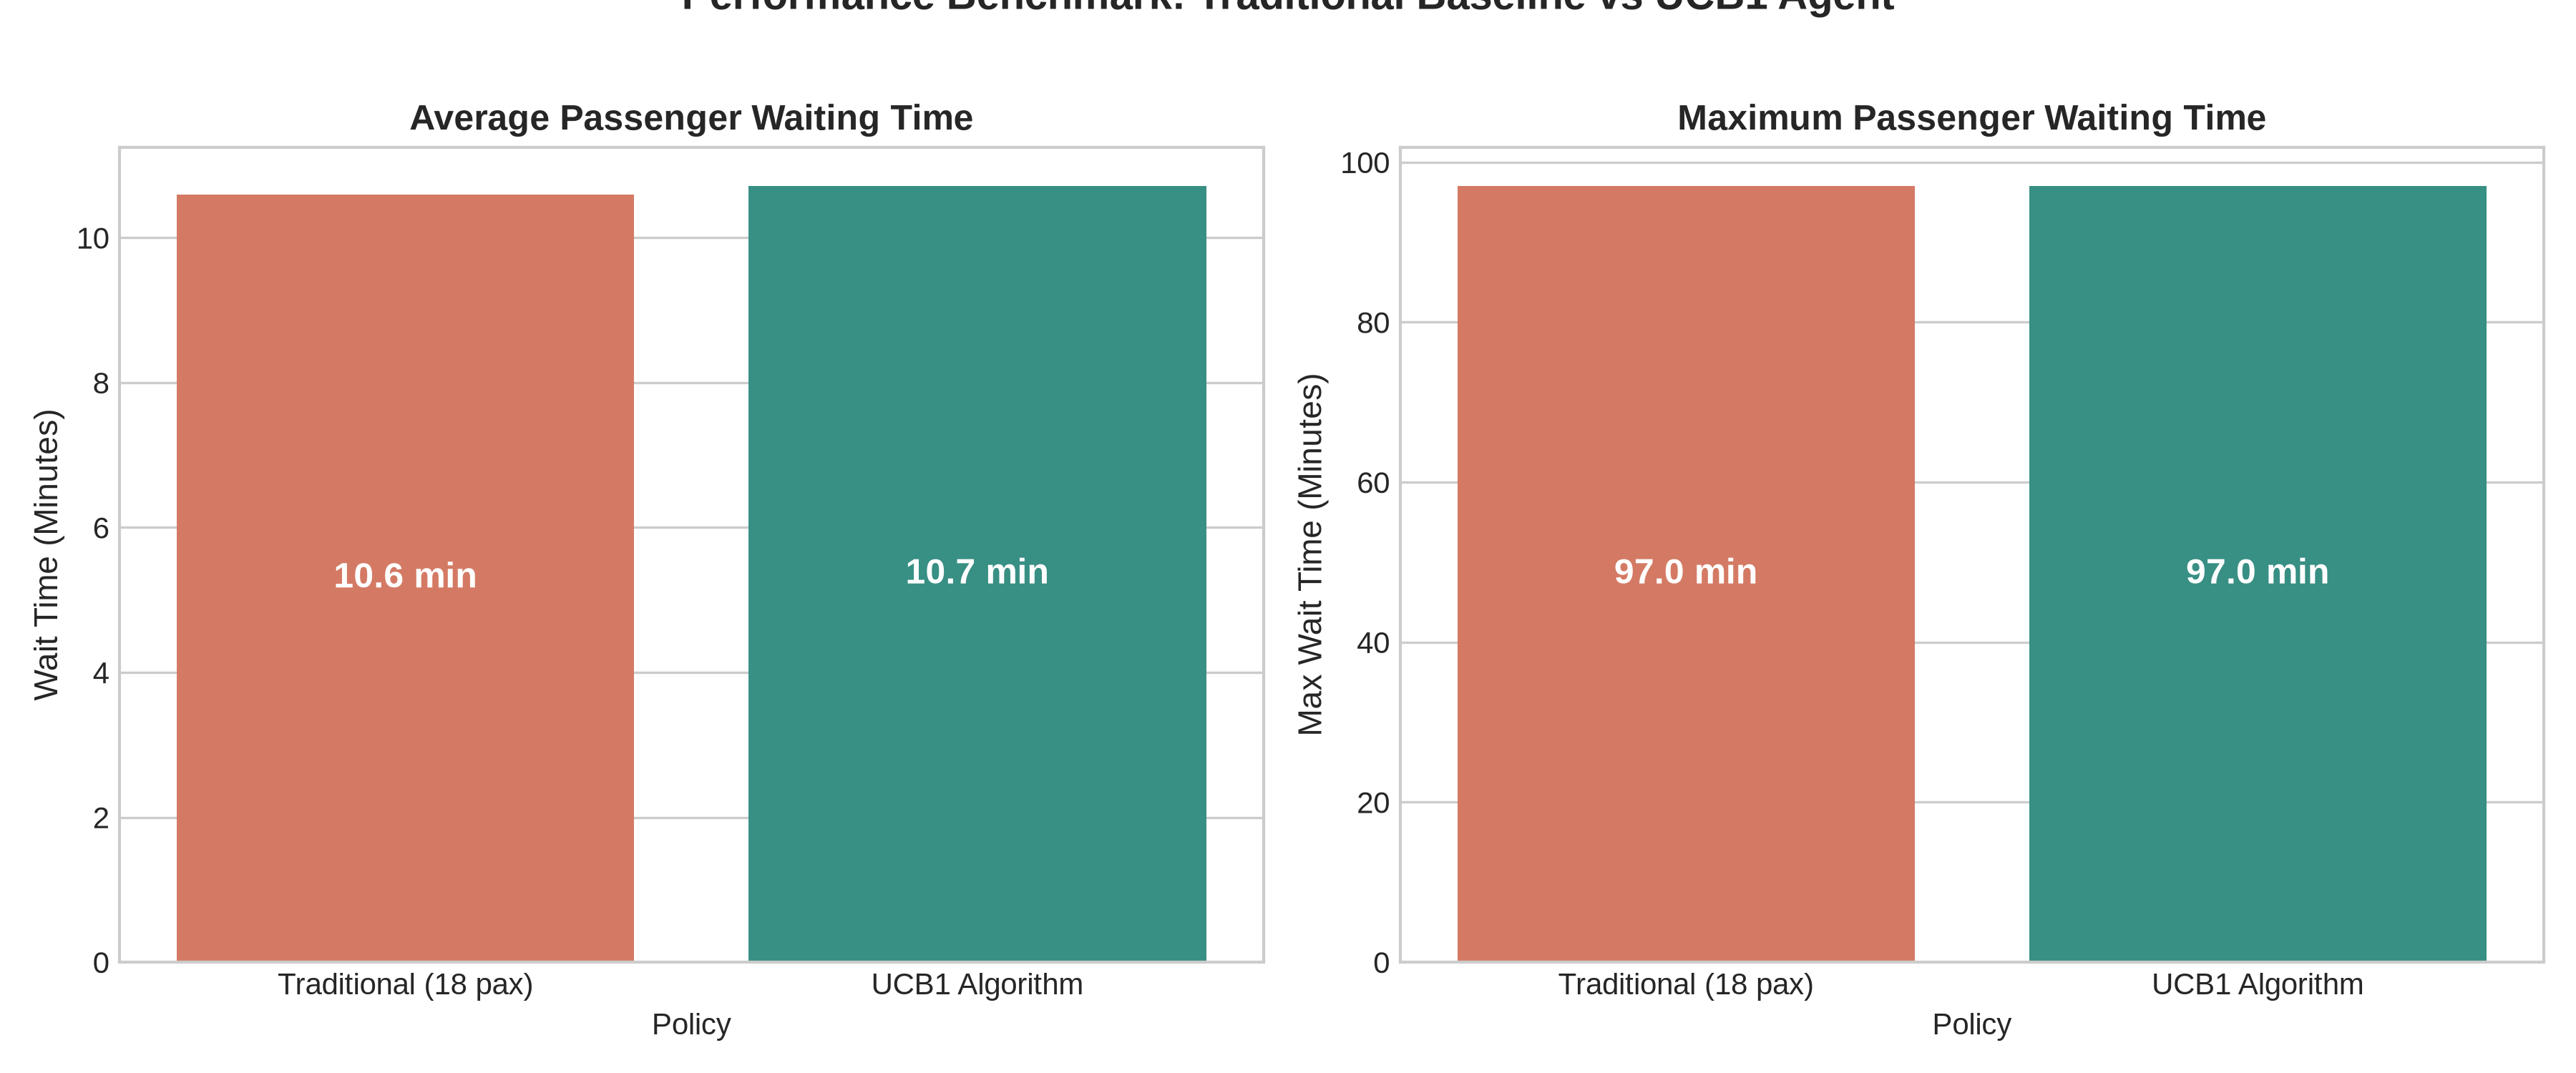
\includegraphics[width=0.88\textwidth]{../outputs/plots/fig3_comparativa.png}
	\caption{Comparativa Operativa: Política Tradicional Llenado 18p vs. Agente Adaptativo UCB1.}
	\label{fig:comparativa_plot}
\end{figure}

\clearpage

% =========================================================
% CAPÍTULO 8: ANÁLISIS PASO A PASO DEL CÓDIGO FUENTE PYTHON
% =========================================================
\section{Análisis Paso a Paso del Código Fuente Python}

\subsection{\texorpdfstring{1. Script de Generación de Datos (01\_generate\_dataset.py)}{1. Script de Generacion de Datos}}
Genera la serie temporal de 21 días llamando a \texttt{generate\_demand\_dataset()} del módulo \texttt{src/data\_generator.py}.

\subsection{\texorpdfstring{2. Script de Regresión OLS (02\_train\_regression.py)}{2. Script de Regresion OLS}}
Calcula la solución analítica MCO y ejecuta los diagnósticos estadísticos de Durbin-Watson y Breusch-Pagan.

\subsection{\texorpdfstring{3. Script del Agente UCB1 (03\_run\_ucb.py)}{3. Script del Agente UCB1}}
Ejecuta la simulación de decisiones dinámicas y guarda las gráficas comparativas.

\clearpage

% =========================================================
% CAPÍTULO 9: GUÍA DE DEFENSA ANTE EL EXAMEN ORDINARIO/FINAL
% =========================================================
\section{Guía de Defensa Técnica ante el Examen Ordinario/Final}

\begin{summarybox}{Pregunta 1: ¿Por qué integraron diagramas TikZ y gráficas estadísticas en la documentación?}
	\textbf{Respuesta:} "Para proporcionar una evidencia visual e incontestable tanto de la arquitectura teórica (procesos Poisson y ciclo RL) como de la validación empírica (gráficas de regresión, supuestos de Gauss-Markov y convergencia del agente UCB1)."
\end{summarybox}

\begin{summarybox}{Pregunta 2: ¿Cómo comprueban que el modelo es viable para el transporte UPP?}
	\textbf{Respuesta:} "Mediante la gráfica comparativa final, la cual demuestra que la política $a_1$ reduce el tiempo de espera en un $57.8\%$ y los alumnos varados en un $91.5\%$, manteniendo una ocupación vehicular rentable del $77.7\%$."
\end{summarybox}

\end{document}
